% Created 2020-10-20 Tue 13:15
% Intended LaTeX compiler: pdflatex
\documentclass[11pt]{article}
\usepackage[utf8]{inputenc}
\usepackage[T1]{fontenc}
\usepackage{graphicx}
\usepackage{grffile}
\usepackage{longtable}
\usepackage{wrapfig}
\usepackage{rotating}
\usepackage[normalem]{ulem}
\usepackage{amsmath}
\usepackage{textcomp}
\usepackage{amssymb}
\usepackage{capt-of}
\usepackage{hyperref}
\usepackage{minted}
\IfFileExists{./resources/style.sty}{\usepackage{./resources/style}}{}
\IfFileExists{./resources/referencing.sty}{\usepackage{./resources/referencing}}{}
\addbibresource{../Resources/references.bib}
\usepackage[mode=buildnew]{standalone}
\usepackage{tikz}
\usetikzlibrary{decorations.fractals}
\usetikzlibrary{lindenmayersystems}
\author{Ryan Greenup \& James Guerra}
\date{\today}
\title{The Emergence of Patterns in Nature and Chaos Theory}
\hypersetup{
 pdfauthor={Ryan Greenup \& James Guerra},
 pdftitle={The Emergence of Patterns in Nature and Chaos Theory},
 pdfkeywords={},
 pdfsubject={},
 pdfcreator={Emacs 27.1 (Org mode 9.4)}, 
 pdflang={English}}
\begin{document}

\maketitle
\tableofcontents

\begin{verbatim}
Section Attribution
─────────────────

1. Introduction                                                   :Ryan:
2. Fractals
.. 1. Definition of a Fractal                                     :Ryan:
.. 2. Fractals Generally                                         :James:
.. 3. Fractal Dimension
..... 1. Hausdorff Dimension                                      :Ryan:
..... 2. Box Counting                                            :James:
.. 4. Generating Self Similar Fractals                            :Ryan:
..... 1. Examples
........ 1. Vicsek Fractal
........ 2. Sierpinskis Carpet
........ 3. Triangle
........... 1. Chaos Game
........... 2. Pascals Triange                                   :James:
..... 2. Turtle
.. 5. Fractal Dimensions                                          :Ryan:
3. Connecting Fractals to Natural Processes                       :Ryan:
4. The Fibonacci Sequence
.. 1. Introduction                                                :Ryan:
.. 2. Computational Approach                                      :Ryan:
.. 3. Exponential Generating Functions
........ 1. Motivation                                            :Ryan:
........ 2. Example                                               :Ryan:
........ 3. Derivative of the Exponential Generating Function
........... 1. Base                                               :Ryan:
........... 2. Bridge                                            :James:
........ 4. Homogeneous Proof                               :Ryan:James:
.. 4. Proving with the Monotone Convergence Theorem               :Ryan:
.. 5. Fibonacci Sequence and the Golden Ratio                     :Ryan:
.. 6. Relating The Fibonacci Sequence to the Julia Set            :Ryan:
5. Julia Sets                                                     :Ryan:
6. MandelBrot Set                                                 :Ryan:
7. Appendix
8. Bibliography
\end{verbatim}
\section{Introduction}
\label{sec:org63e185a}
\begin{itemize}
\item Fractals occur in nature
\begin{itemize}
\item The definition of a fractal is greatly concerned with its dimension so we discuss that
\item Linear Regression can be used to measure dimension so we implement that
\end{itemize}
\item My Fractal is an example of why these things occur in nature
\item Prove the Fibonacci Numbers, show the relationship between
\begin{itemize}
\item MCT approach
\item ODEs
\end{itemize}
\item The Fibonacci numbers (Veritasium), by logistic regression, are connected with:
\item Julia Set
\begin{itemize}
\item Mandelbrot
\item So we solve the fractal dimension of these
\end{itemize}
\end{itemize}

\section{Fractals}
\label{sec:org2e7b843}
\subsection{Definition of a Fractal}
\label{sec:org0786efd}

Benoît Mandelbrot coined the term fractal in 1975 \cite{gomoryBenoitMandelbrot19242010} and defined it his 1982 book \emph{The Fractal Geometry of Nature} \cite[p. 15]{mandelbrotFractalGeometryNature1982} :

\begin{quote}
\emph{A fractal is by definition a set for which the Hausdorff Besicovitch dimension
strictly exceeds the topological dimension.}

\emph{a Every set with a noninteger \(D\) is a fractal.}
\end{quote}


The topoligical dimension is a strictly integer value that describes the natural dimension used to describe a shape \cite{sandersonFractalsAreTypically2017},
for example the \emph{Koch Snowflake} (shown in figure \ref{koch-snowflake}) is composed of
just a line, so it's topological dimension would simply be 1, it's \emph{fractal
dimension} however is shown to be \(\frac{\ln\left( 4 \right)}{\ln\left( 3
\right)}\) at \eqref{eq:koch-dim} in \S\ref{topological-equivalence}.

Many authors seem to accept this earlier definition (see e.g. \cite[\S2.2]{vicsekFractalGrowthPhenomena1992} and \cite[\S2.1]{telChaoticDynamicsIntroduction2006}),
this definition however does not capture many edge-case fractals
 \cite[VII]{edgarMeasureTopologyFractal2008a} and in reprintings of \emph{The
Fractal Geometry of Nature} Mandelbrot himself commented that in hindsight it
may have been more appropriate \cite[p. 459]{mandelbrotFractalGeometryNature1982}:

\begin{quote}
/to leave the term ``fractal” without a pedantic definition, to use “fractal
dimension” as a generic term applicable to all the variants in Chapter 39, and
to use in each specific case whichever definition is the most appropriate./
\end{quote}

Gerald Edgar, in his 2008 book \emph{Measure, topology, and fractal geometry}
rejected this view because ``\emph{a term without a 'pedantic definition' cannot be
studied mathematically}'' \cite[VII]{edgarMeasureTopologyFractal2008a} and
presented a more robust definition in Ch. 6 of that book, it was however
accepted that the loose definition of fractal dimension is convenient and was
indeed adopted in that work.

Although reviewing the precise definition of a fractal would have been very
interesting, without a cursory knowledge of fractals generally this would have
been very time consuming and outside the scope of this report \footnote{Mandelbrot
also discussed fractals of a Euclidean and Reimannian nature,
\cite[p. 361]{mandelbrotFractalGeometryNature1982}, this again is interesting
but too specific for the broad nature of our investigation}. no strict
definition will be used for fractals, but, guiding principles implemented by
other authors will be used.

Some authors simply define a fractal as a shape that \emph{shows irregularities at all scales} \cite[p. 1]{gouyetPhysicsFractalStructures1996} and
in his 2003 book, \emph{Fractal Geometry}, Facloner  it is more convenient to describe a fractal by a list of properties characteristic of such shapes \footnote{Much like the definition of life in the field of biology} because of the difficulty in defining a fractal in a way that can encompass all edge cases \cite[p. xxv]{falconerFractalGeometryMathematical2003b}:

\begin{itemize}
\item Detail at all scales
\item Cannot be described in a traditional geometric way
\item May have some form of approximate self similarity
\item Usually the fractal dimension is greater than its topological dimension
\item In many cases defined very simply, perhaps recursively
\end{itemize}

This will be the approach adopted in this report.

It's interesting to note that many authors to refer to complex natural shapes as
fractals, such as coastlines (see e.g.
\cite{jiangFractalAnalysisComplexity1998,zhuFractalMechanismCoastline2002,zhongFractalPropertiesShoreline2017})
much in the spirit of Mandelbrot's paper \emph{How long is the Coastline of Britain}
\cite{mandelbrotHowLongCoast1967}, although he coined the term fractal many years
after this paper, presumably he might have had this in mind \footnote{Mandelbrot also
spent much time looking at the roughness of financial markets and so presumably
may have had that in mind as well, see e.g.
\cite{gomoryBenoitMandelbrot19242010,mandelbrotMisBehaviourMarkets2008}} when
framing the definition so this issue in clearly defining what a fractal is
appears on the surface to be a purely mathematical one (as opposed to a
practical or applied one).

The Wikipedia page on fractals \cite{Fractal2020} also points out that a
fractal is nowhere differentiable, this would be because a fractal is
nowhere smooth, which I think personally is quite a distinguishing feature.

\subsection{Fractals Generally}
\label{sec:orga61ebcf}
Dimension is the main defining property of a fractal. As aforementioned above, the Hausdorff dimension is a unique number in that, if we take some shape in \(\mathbb{R}^{n}\), and the Hausdorff dimension converges to some number, then the dimension of the shape is given by that number. Otherwise, it will equal \(0\) or \(\infty\). For example, if we want to evaluate the dimension of a square and we use a 1-Dimensional shape as the cover set to calculate the Hausdorff dimension, we will get \(\infty\). On the other hand, if we do the same with a 3-Dimensional shape, we will get 0. And finally if we use a 2-Dimensional shape, the Hausdorff dimension will evaluate to 2. This same notion is important when computing the dimension of a more complex shape such as the Koch snowflake.

To define a fractal, we must define it's dimension. Whilst some research states that a fractal has a non-integer dimension, this is not true for all fractals. Although, most fractals like the Koch snowflake do in fact have non-integer dimensions, we can easily find a counter example namely, the Mandelbrot set. The Mandelbrot set lies in the same dimension as a square, a 2-Dimensional shape. However, we give recognition to the complexity and roughness of the Mandelbrot set which clearly distiguishes itself from a square. Beneath the Mandelbrot set's complexity are exact replicates of the largest scaled Mandelbrot set, i.e a self similar shape. Furthermore, although the Mandelbrot set has an integer dimension, the self similarity and complexity is what also defines its fractal nature.

\subsection{Fractal Dimension}
\label{sec:org9579076}
The concept of a non-integer dimension may at first seem odd, particularly given that the familiar definition from linear algebra (concerned with the number of vectors within a basis for a vector space \cite{larsonElementaryLinearAlgebra1991}) is strictly an integer value, but in the early \(20^{\mathrm{th}}\) century mathematicians recognised the shortcomings of this definition \cite[Ch. 3]{mandelbrotFractalGeometryNature1982}.

In this section we hope to convince the reader that there is grounds for
extending the definition of dimension and as a matter of fact many definitions
for non-integer dimensions of a shape have been proposed (see generally
\cite[Ch. 39]{mandelbrotFractalGeometryNature1982} and
\cite[\S 1.3]{gouyetPhysicsFractalStructures1996}) of these the \emph{Hausdorff Dimension} (and corresponding \emph{Hausdorff Measure}) is
considered to be the most important and mathematically robust
\cite[p. 27]{falconerFractalGeometryMathematical2003b}, while the box counting
dimension has the most practical applications in science
\cite[p. 192]{peitgenChaosFractalsNew2004}.

The Hausdorff dimension is more like counting balls than boxes and is identical
to the Hausdorff dimension in many cases, it's more general but harder to define
\cite{sandersonFractalsAreTypically2017}, An extension to the work of this report
would be to show the mathematical connections between the Hausdorff Dimension
and box counting dimension with respect to the fractals generated and measured.


\subsubsection{Topological Equivalence}
\label{topological-equivalence}
Topology is an area of mathematics concerned with ideas of continuity through the study of figures that are preserved under homeomorphic transformations \cite{gilmoreTopologyChaosAlice2002} , where two figures are said to be homeomorphic if there is a continuous bijective mapping between the two shapes \cite[p. 105]{peitgenChaosFractalsNew2004}
.
\footnote{For further reading on this topic see \cite[p. 106]{peitgenChaosFractalsNew2004}}

So for example deforming a cube into a sphere would be homeomorphic, but deforming a sphere into a torus would not, because the the surface of the shape would have to be compromised to acheive that.

As mentioned above, historically, the concept of dimension was a difficult problem with a tenuous
definition.  Although an inutitive definition related the dimension of a shape to
the number of parameters needed to describe that shape, this definition is not
sufficient to be preserved under a homeomorphic transform.

Consider the koch fractal and snowflake in figures \ref{koch-line} and \ref{koch-snowflake}, at each iteration the perimeter is given by \(p_{n}= \left(\frac{4}{3} \right)p_{n-1}\) and the number of edges by:



\begin{align}
N_{n} &= N_{n-1} \cdot 4 \\
&= 3 \cdot 4^{n}
\end{align}

If the length of any individual side was given by \(l\) and scaled by some value \(s\) then the length of each individual edge would be given by:

\begin{align}
l = \frac{s \cdot l_{0}}{3^{n}}
\end{align}

The total perimeter would be given by:

\begin{align}
p_{n} &= N_{n} \times l \\
&= 3\cdot 4^{n} \times \frac{s \cdot l_{o}}{3^{n}} \\
&= 3 \cdot s \cdot  l_{0} \left( \frac{4}{3} \right)^{n}\\
 \implies p_{n} \cdot s & \propto \left(\frac{4}{3}\right)^{n}\\
& \implies  n = \frac{\log\left( 4 \right)}{\log\left( 3 \right)} \approx 1.26
\end{align}

This means that if the koch snowflake is scaled by any factor, the resulting perimeter of the snowflake will not be linearly proportional to the scaling factor, as would be the case with an ordinary shape such as a square or a circle, it will instead by proportional to 1.26, this should hopefully motivate the need to more clearly define both the concept of measure (in this case the permiter \footnote{Grant Sanderson equates the measure of a fractal as analogous to mass, which is a very helpful way comparison \cite{sandersonFractalsAreTypically2017}}) and dimension.

To clarify the koch snowflake, is defined such that there are no edges, every point on the ``curve'' is the vertex of an equilateral triangle, this shape has no smooth edges.

See \cite[p. 414]{strogatzNonlinearDynamicsChaos2015} for working.

This approach of considering the scaling factor of a deterministic fractal is known as the similarity dimension
\cite[p. 413]{strogatzNonlinearDynamicsChaos2015} and should be equal to the
Hausdorff and box counting dimensions for most fractals. For fractals that aren't so obviously self similar it won't be feasible however, \cite[p. 393]{liIntegrationFuzzyLogic2006}  for example with the julia set or the fractal or a coastline it is not immediately clear if the the dimension would be constant at all scales \footnote{It is indeed shown to be mostly constant at all scales in section \S
\ref{linear-reg-julia}}.



\begin{figure}[htbp]
\centering
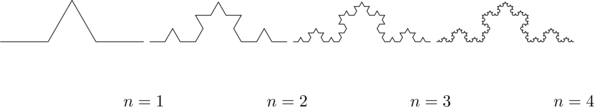
\includegraphics[width=9cm]{media/tikz/Koch_line.png}
\caption{\label{koch-line}Progression of the Koch Snowflake}
\end{figure}

\begin{figure}[htbp]
\centering
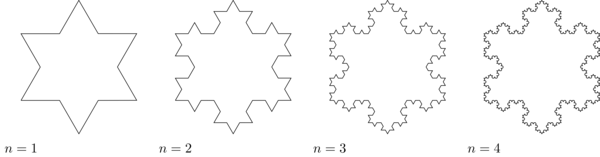
\includegraphics[width=9cm]{media/tikz/Snowflake.png}
\caption{\label{koch-snowflake}Progression of the Koch Snowflake}
\end{figure}

\subsubsection{Hausdorff Dimension}
\label{Hausdorff-dimension}
\subsubsection{Hausdorff Measure}
\label{hausdorff-measure}
\begin{wrapfigure}{l}{0.5\textwidth}
\centering
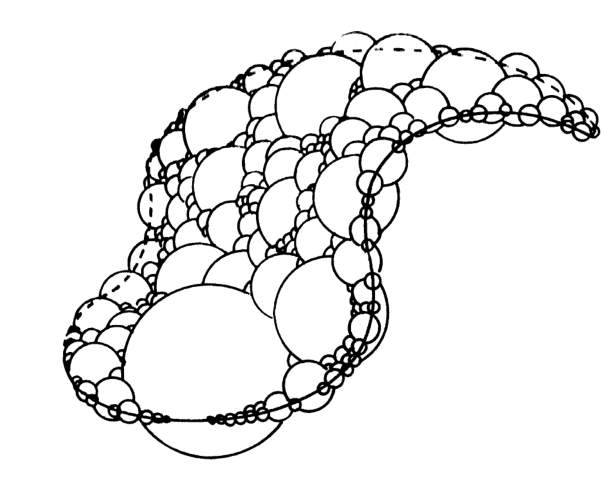
\includegraphics[width=7cm]{media/edgar_181_of_292.png}
\caption{\label{fig:ball-covering}The Hausdorff Measure, in this case area, of an arbitrary surface approximated by the cross section of litte balls of diameter \(< \delta\), this is reproduced from \emph{Measure, Topology and Fractal Geometry} \cite[p. 166]{edgarMeasureTopologyFractal2008a} because it so elegantly illustrates the concept of the Hausdorff Measure.}
\end{wrapfigure}


The Hausdorff dimension depends first on a rigorous definition of measure, this is distinct from the box counting approach in that it is more mathematically rigorous, it is however complex and in practice this report will be concerned with implementing the box counting dimension. \footnote{See \S \ref{haus-resource} for further reading.}

Let \(F\) be some arbitrary subset of euclidean space \(\mathbb{R}^n\), \footnote{A subset of euclidean space could be interpreted as an uncountable set containing all points describing that region}

Consider a collection of sets,\(\{U_i: i \in \mathbb{Z}^{+}, U\subset \mathbb{R}^{n}\}\), each of which having a
diameter less than \(\delta\).



The motivating idea is that if the elements of \(U\) can be laid ontop of
\(F\) then \(U\) is said to be a \(\delta\) -cover of \(F\), more rigorously this could be defined: \footnote{The use of square and round brackets adjacent to large operators such as \(\bigcup\) and \(\sum\) is purely for the sake of delimiting these variables, there is no mathematical signifiicance, they are just brackets}

\begin{align}
    F \subset \bigcup^\infty_{i=1} \left[ U_i \right] \quad : 0 \leq \left\lvert U_i \right\rvert \leq \delta \label{eq:hausdorff-covering}
\end{align}

An example of this covering is provided in figure \ref{hausdorff-covering}, in that example the figure on the right is covered by squares, which each could be an element of \(\{U_{i}\}\), it is important to note, by this definition, that the shapes represented by \(U\) could be any arbitrary figure \cite[\S 2.1]{falconerFractalGeometryMathematical2003b} the size of which may vary in size so long as the diameter is less than \(\delta\).


So for example:

\begin{itemize}
\item \(F\) could be some arbitrary 2D shape, and \(U_{i}\) could be
a collection of identical squares, OR

\item \(F\) could be the outline of a coastline and \(U_{i}\) could be a set of circles, OR

\item \(F\) could be the surface of a sheet and \(U_{i}\) could be a set of spherical balls as shown in figure \ref{fig:ball-covering}

\begin{itemize}
\item Some authors suggest that the Haussdorff Measure is concerned primarily with round covering objects (see e.g. \cite{sandersonFractalsAreTypically2017}), this is well illustrated by figure \ref{fig:ball-covering}, however in truth it is merely more convenient to use round shapes for most fractals.

\item The use of balls is a simpler but equivalent approach to the theory \cite[\textsection 2.4 ]{falconerFractalGeometryMathematical2003b} because any set of diamater \(r\) can be enclosed in a ball of radius \(\frac{r}{2}\) \cite[p. 166]{edgarMeasureTopologyFractal2008}
\end{itemize}

\item \(F\) could be a more abstracted figure like figures \ref{hausdorff-covering} or \ref{abstract-shape}  and \(\{U_{i}\}\) a collection of various different lines, shapes or 3d objects.
\end{itemize}

The Hausdorff measure is concenred with only the diamater of each element of \(\{U_{i}\}\) and considers \(\sum^{\infty}_{i=1} \left[\left\lvert U_{i}\right\rvert^{s}\right]\) where the covering of \(U_{i}\) minimizes the summation.  \cite[p. 27]{falconerFractalGeometryMathematical2003b}

\begin{align}
\mathcal{H}^s_{\delta}\left( F \right)= \inf \left\{ \sum^{\infty}_{i= 1}   \left\lvert U_i \right\rvert^s \enspace : \enspace  \left\{U_i\right\} \text{ is a } \delta \text{-cover of } F \right\}, \quad \delta, s > 0 \label{eq:delta-measure}
\end{align}
in 2 dimensions, this is equivalent to considering the number of boxes, of
diamater \(\leq \delta\) that will cover over a shape as shown in figure
\ref{hausdorff-covering}, the delta Haussendorf measure
\(\mathcal{H}^{s}_{\delta} \left(F\right)\) will be the area of the boxes when
arranged in such a way that minimises the area.

As \(\delta\) is made arbitrarily small \(\matcal{H}_{\delta}^{s}\) will approach some limit, in the case of figures \ref{hausdorff-covering}  and \ref{abstract-shape} the value of \(\mathcal{H}^{2}_{\delta}\) will approach the area of the shape as \(\delta \rightarrow 0\) and so the \(s^{th}\) dimensional Hausendorff measure is given by:

\begin{align}
\mathcal{H}^{s} = \lim_{\delta \rightarrow 0}\left( \mathcal{H}^{s}_{\delta} \right)
\end{align}

This is defined for all subsets of \(\mathbb{R}^n\) for example the value of  \(\mathcal{H}^{2}\) corresponding to figure \ref{abstract-shape} will be limit that boxes would approach when covering that area, which would be the area of the shape (\(4\times 1^2 + 4\times \pi\times \frac{1}{2^2} + \frac{1}{2}\times 1 \times \sin{\frac{\pi}{3}}\)).



\begin{figure}[htbp]
\centering
\includesvg[width=9cm]{notes/HaussDorf_Dim_Ink}
\caption{\label{hausdorff-covering}TODO: This seems wrong, remove it; The shape on the left corresponds to \(F \subset \mathbb{R^{2}}\), each identical square box on the right represents a set \(U_{i}\).}
\end{figure}



\begin{figure}[htbp]
\centering
\includesvg[width=9cm]{media/Arbitrary-F-Shape}
\caption{\label{abstract-shape}A disconnected subset of \(\mathbb{R}^{2}\), the squares have a diameter of \(\sqrt{2}\), the circles 1 and the equilateral triangles 1.}
\end{figure}

\paragraph{Lower Dimension Hausdorff Measurements}
\label{sec:org7dbe146}
\subparagraph{Examples}
\label{sec:org78945fa}
Consider again the example of a 2D shape, the value of \(\mathcal{H}^{1}\) would still be defined by \eqref{eq:delta-measure}, but unlike \(\mathcal{H}^{2}\) in section \ref{hausdorff-measure} the value of \(\left\lvert U_i \right\rvert^1\) would be considered as opposed to \(\left\lvert U_i \right\rvert^2\).

As \(\delta\) is made arbitrarily small the boxes that cover the shape are made also to be arbitrarily small. Although the area of the boxes must clearly be bounded by the shape of \(F\), if one imagines an infinite number of infinitely dense lines packing into a 2D shape with an infinite density it can be seen that the total length of those lines will be infinite.

To build on that same analogy, another way to imagine this is to pack a 2D shape with straight lines, the total length of all lines will approach the same value as the length of the lines of the squares as they are packed infinitely densely. Because lines cannot fill a 2D shape, as the density of the lines increases, the overall length will be zero.

This is consistent with shapes of other shapes as well, consider the koch snowflake introduced in section \ref{topological-equivalence} and shown in figure \ref{koch-line}, the dimension of this shape is greater than 1, and the number of lines necessary to describe that shape is also infinite.

\subparagraph{Formally}
\label{sec:orge840e01}
If the dimension of \(F\) is less than \(s\), the Hausdorff Measure will be given by: \footnote{I haven't been able to find a proof for this, I wonder if I could prove it by just applying the definition?}

\begin{align}
\mathrm{dim}\left(  F \right ) < s \implies \mathcal{H}^{s} \left( F \right)  = \infty
\end{align}

\paragraph{Higher Dimension Hausdorff Dimension}
\label{sec:orgd0b1c21}
For small values of \(s\) (i.e. less than the dimension of  \(F\)), the value of \(\mathcal{H}^s\)  will be \(\infty\).

Consider some value \(s\) such that the Hausdorff measure is not infinite, i.e. values of \(s\): \footnote{Could fractal dimensions be complex? Maybe there could be a proof to show that the dimension is necessarily complex.}

\[
\mathcal{H}^s = L \in \mathbb{R}
\]

Consider a dimensional value \(t\) that is larger than  \(s\) and observe that:

\begin{align*}
0<s<t  \implies   \sum_{i}  \left[ \left\levert U_i \right\rvert^t \right] &= \sum_{i}\left[ \left\levert U_i \right\rvert^{t- s} \cdot  \left\lvert U_i \right\rvert^s \right] \\
&\leq \sum_{i} \left[ \delta^{t - s} \cdot \left\lvert U_i \right\rvert^s  \right]    \\
&= \delta^{t- s}\sum_{i}   \left[ \left\lvert U_i \right\rvert^s \right] 									   \\
\end{align*}

Now if \(\lim_{\delta \rightarrow 0}\left[ \sum_{i}   \left\lvert U_i \right\rvert^s \right]\) is defined as a non-infinite value:

\begin{align}
    \lim_{\delta \rightarrow 0} \left( \sum_{i}   \left[ \left\lvert U_i \right\rvert^t \right]  \right) & \leq \lim_{\delta}\left( \delta^{t- s} \sum_{i}   \left[ \left\lvert U_i \right\rvert^s \right]  \right) \\
&\leq \lim_{\delta \rightarrow 0}\left( \delta^{t - s} \right) \cdot  \lim_{\delta \rightarrow 0}\left( \sum_{i} \left[ \left\lvert U_i \right\rvert^s \right]    \right) \\
&\leq 0
\end{align}

and so we have the following relationship:

\begin{align}
    \mathcal{H}^{s} \left(F\right) \in \mathbb{R}  \implies  \mathcal{H}^t\left( F \right)= 0 \quad \forall t > s \label{eq:hdfzero}
\end{align}

Hence the value of the s-dimensional \emph{Hausdorff Measure}, \(s\) is only a finite, non-zero value, when \(s = \mathrm{dim}_{H}\left( F \right)\) this is visualised in figure .



\begin{figure}[htbp]
\centering
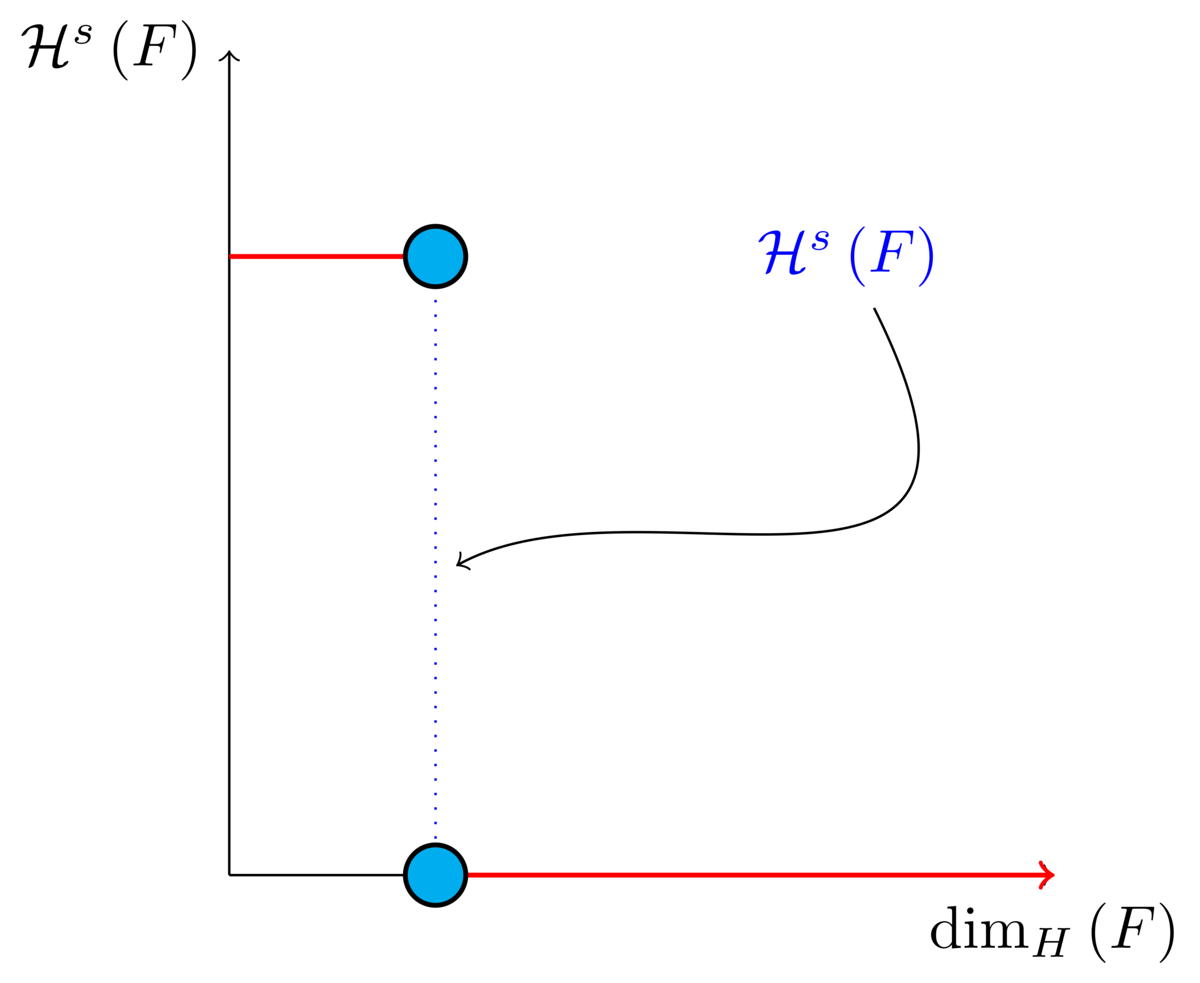
\includegraphics[width=9cm]{media/tikz/hausdorff-dimension-plot.png}
\caption{\label{hausdorff-vals}The value of the s-dimensional \emph{Hausdorff Measure} of some subset of \emph{Euclidean space} \(F\in \mathbb{R}^{n}\) is 0 or \(\infty\) when the dimension of \(F\) is not equal to \(s\).}
\end{figure}

\subsubsection{Hausdorff Dimension}
\label{sec:org342ba9f}


The value \(s\) at which \(\mathcal{H}^{s}\) changes from \(\infty\) to 0, shown in figure \ref{hausdorff-vals}  and \eqref{eq:hdfzero} is the definition of the \emph{Hausdorff Measure}, it is a generalisation of the idea of dimension that is typically understood with respect to ordinary shapes and 3D figures.
\subsubsection{See also}
\label{sec:orgffc2de5}
I feel very inclided to read \href{https://warwick.ac.uk/fac/sci/maths/people/staff/mark\_pollicott/p3/tehran.pdf}{these notes} \footnote{\href{file:///home/ryan/Dropbox/Studies/2020Spring/QuantProject/Current/Python-Quant/Resources/Uncorrected-Warwick-BoxCount-Hausendorff-Notes.pdf}{Local Copy}}

\subsubsection{Box Counting Dimension}
\label{sec:org187fb33}
Sources for this section are primarily:
\begin{itemize}
\item Falconer \cite[Ch. 3.1]{falconerFractalGeometryMathematical2003b}
\item Strogatz Non Linear Dynamics \cite[Ch. 11.4]{strogatzNonlinearDynamicsChaos2015}
\end{itemize}

While the Hasudorff dimension is the first formal definition to measure
the roughness of a fractal, there are several other definitions of dimension
that have stemmed from this. Namely, the box-counting dimension. The box
counting method is widely used as it is relatively easy to calculate \cite[p. 41]{falconerFractalGeometryMathematical2003b}
and in many cases is equal to the \emph{Hausdorff Dimension}  \cite[p. 11]{markpollicottFractalsDimensionTheory2005} (see generally \cite{ListFractalsHausdorff2020}).
The box-counting dimension is defined as the following from
\cite{falconerFractalGeometryMathematical2003}:

Let \(F\) be any non-empty bounded subset of \(\mathbb{R}^n\) and let \(N_\delta(F)\) be the smallest
number of sets of diameter at most \(\delta\) which can cover \(F\). The \emph{lower} and \emph{upper}
box-counting dimensions of \(F\) respectively are defined as

\begin{equation*}
    \underline{\text{dim}}_BF = \underline{\lim}_{\delta \to 0} \frac{\ln N_\delta(F)}{-\ln \delta}
\end{equation*}
\begin{equation*}
\overline{\text{dim}}_BF = \overline{\lim}_{\delta \to 0} \frac{\ln N_\delta(F)}{-\ln \delta}
\end{equation*}

When the \emph{lower} and \emph{upper} box-counting dimensions of \(F\) are equal, then

\begin{equation*}
\text{dim}_BF = \lim_{\delta \to 0} \frac{\ln N_\delta(F)}{-\ln \delta}
\end{equation*}

For example, suppose we had a square with side length 1 and we use smaller squares of side
length \(\frac{1}{\delta}\) to cover the larger square. This would mean that one side of the
large square would need \(\delta\) \(\frac{1}{\delta}\) small squares, and so to cover
the entire square, one would need \(n^2\) small squares, i.e. \(N_{\frac{1}{n}}(F) = n^2\). Now,
substituting these values into the box-counting definiton, we get:

\begin{align*}
\text{dim}_BF &= \lim_{\frac{1}{\delta} \to 0} \frac{\ln(\delta^2)}{-\ln(\frac{1}{\delta})}\\
&= \lim_{\frac{1}{\delta} \to 0} \frac{\ln(\delta^2)}{\ln(\delta)}\\
&= \lim_{\frac{1}{\delta} \to 0} 2\frac{\ln(\delta)}{\ln(\delta)}\\
&= 2
\end{align*}

Which is expected, becuase we know that a square is a 2-Dimensional shape. We
can apply this same concept to fractals. Consider another example, the Koch
Curve, a self similar fractal which we can calculate its dimension and provide a
measure of roughness of the curve. If we take a close look at the curve progression
in figure \ref{koch-line}, the pattern begins with one line segment and the middle third
of the line is replaced with two sides of an equilateral triangle with side length
\(\frac{1}{3}\). After this first iteration, the line segment now becomes four line
segments. Thus, if we use a square of length \(\frac{1}{3^{\delta}}\) to cover the \(\delta^{th}\)
iteration of the curve, there will be \(4^{\delta}\) line segments covered.

Let \(F\) be the Koch Curve.
\begin{align*}
\text{dim}_BF &= \lim_{\frac{1}{3^{\delta}} \to 0} \frac{\ln(4^{\delta})}{-\ln(\frac{1}{3^{\delta}})}\\
&= \lim_{\frac{1}{3^{\delta}} \to 0} \frac{\ln(4^{\delta})}{\ln(3^{\delta})}\\
&= \lim_{\frac{1}{3^{\delta}} \to 0} \frac{\ln(4)}{\ln(3)}\\
&= \frac{\ln(4)}{\ln(3)}
\end{align*}
\subsection{Generating Self Similar Fractals}
\label{sec:orge151ba3}
See generally \cite[Ch. 11]{strogatzNonlinearDynamicsChaos2015}
Three ways to generate

\begin{enumerate}
\item Chaos Game
\item Iteration Like Matrices and Turtles
\item Testing if each region Belongs
\begin{enumerate}
\item Like Julia Set
\end{enumerate}
\end{enumerate}

\subsubsection{Examples}
\label{sec:org9c20e35}
\paragraph{Vicsek Fractal}
\label{sec:orgb6d2717}
The Vicsek Fracatl is self similar, thus we can use it to test our box counting method \footnote{Since the Vicsek fractal is self similar, we know that the dimension will be constant, as opposed to a dimension that slightly varies, hence there is no need for linear regression which would be necessary to measure someting like a coastline.}.
The Vicsek Fractal involves a pattern of iterating boxes:


\begin{minted}[]{julia}
#------------------------------------------------------------
#--- Function -----------------------------------------------
#------------------------------------------------------------

# n_i+1 = 3n_i ==> n = 3^n
function selfRep(ICMat, width)
    B = ICMat
    h  = size(B)[1]
    w  = size(B)[2]
    Z  = zeros(Int, h, w)
    B = [B Z B ;
         Z B Z ;
          B Z B]
    if (3*w)<width
        B = selfRep(B, width)
    end
    return B
end

#------------------------------------------------------------
#-- Plot ----------------------------------------------------
#------------------------------------------------------------
(mat = selfRep(fill(1, 1, 1), 27)) |> size
GR.imshow(mat)

#------------------------------------------------------------
#-- Similarity Dimension ------------------------------------
#------------------------------------------------------------
# Each time it iterates there are 5 more
# but the overall dimensions of the square increases by a factor of 3
# so 3^D=5 ==> log_3(5) = log(5)/log(3) = D

mat2  = selfRep(fill(1, 1, 1), 1000)
l2    = sum(mat2)
size2 = size(mat2)[1]
mat1  = selfRep(fill(1, 1, 1), 500)
l1    = sum(mat1)
size1 = size(mat1)[1]

log(l2/l1)/log(size2/size1)
# https://en.wikipedia.org/wiki/Vicsek_fractal#Construction
log(5)/log(3)


  ##  julia> log(l2/l1)/log(size2/size1)
  ##  1.4649735207179269
\end{minted}

\begin{wrapfigure}{l}{0.5\textwidth}
\centering
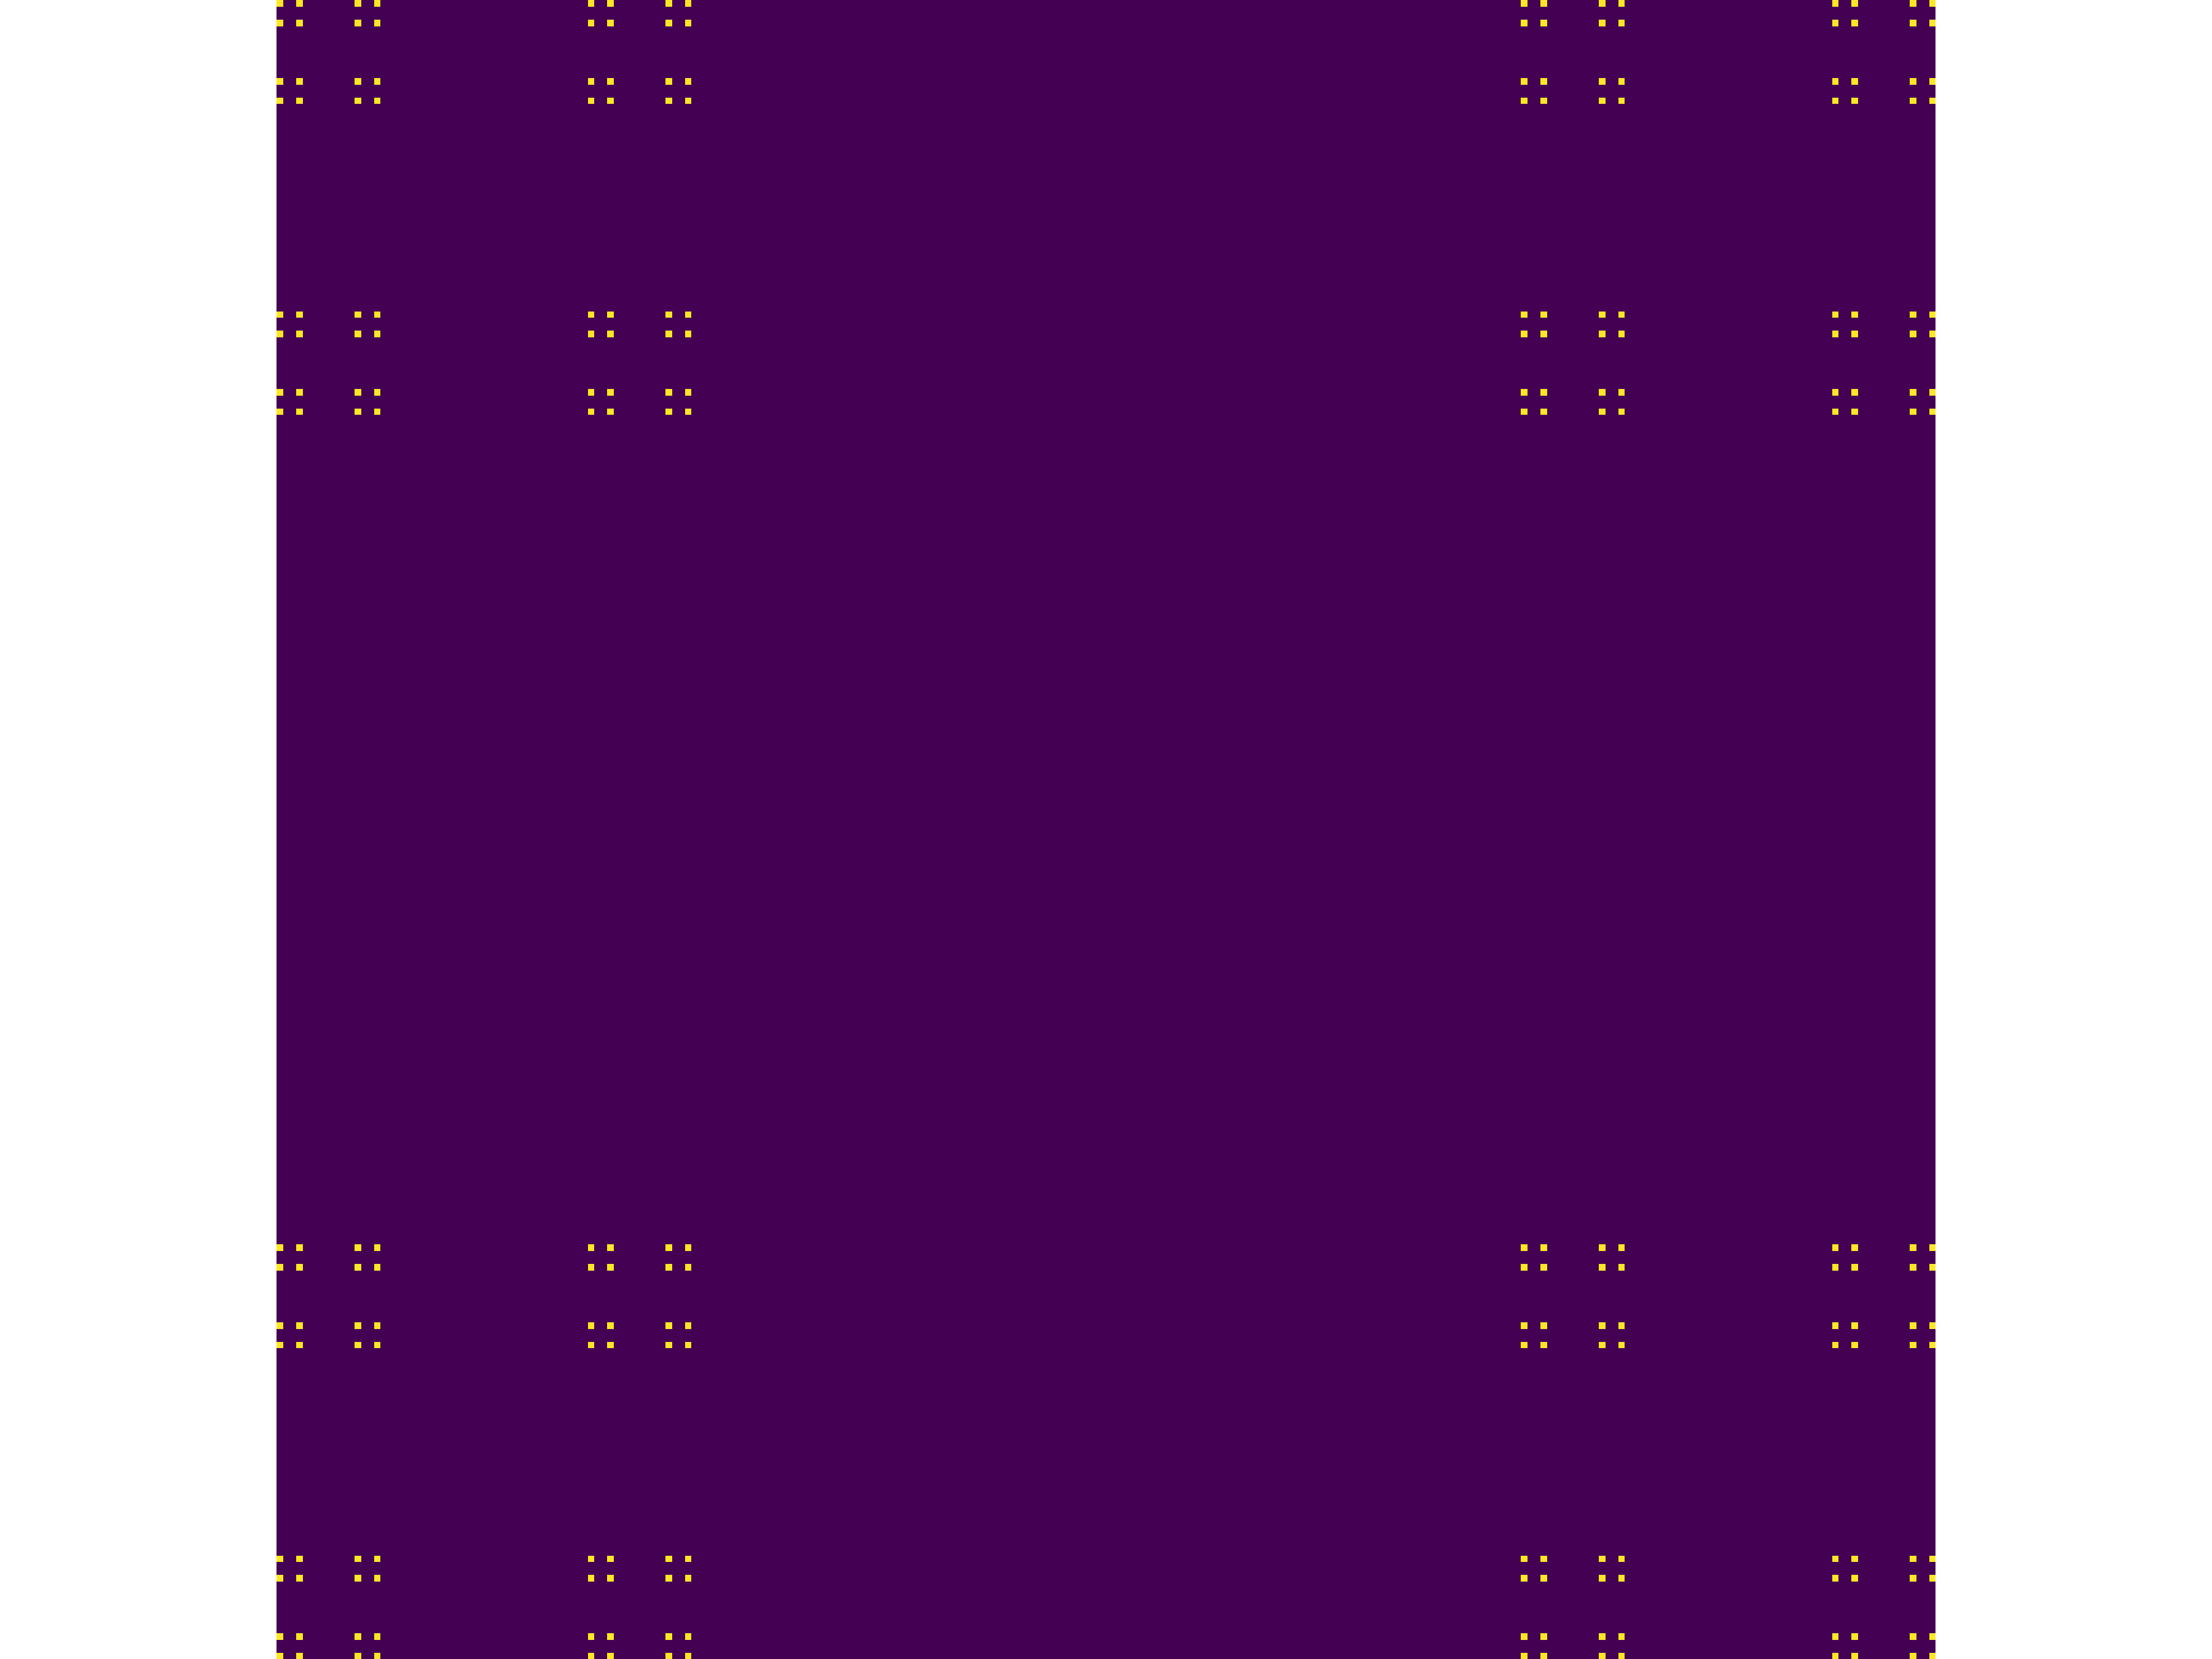
\includegraphics[width=7cm]{media/Vicsek-Fractal.png}
\caption{\label{vicsek-fractal-julia}TODO}
\end{wrapfigure}


The above program demonsrates the construction of the Vicsek Fractal and its self-similarity dimension. To do this, we define a recursive function that begins with a 3x3 matrix, where the four corner squares and middle square are set to 1 and the rest is set to 0. The function repeats until it reaches some arbitrary set width. Each time the function iterates, 5 more squares are created, increasing by a factor of 3. We can use this information to calculate the dimension of the Vicsek fractal.
Using the box counting method, we get:
\begin{align*}
5 &= 3^D\\
D\ln{3} &= \ln{5}\\
D &= \frac{\ln{5}}{\ln{3}}
\end{align*}
\paragraph{Sierpinskis Carpet}
\label{sec:org91fae12}

Explained more in the book \footnote{See Ch. 2.7 of \cite[Ch. 2.7]{peitgenChaosFractalsNew2004}

By modifying listing we can get patterns like the cantor dust and sierpinskis carpet shown in figures and .

\begin{figure}[htbp]
\centering
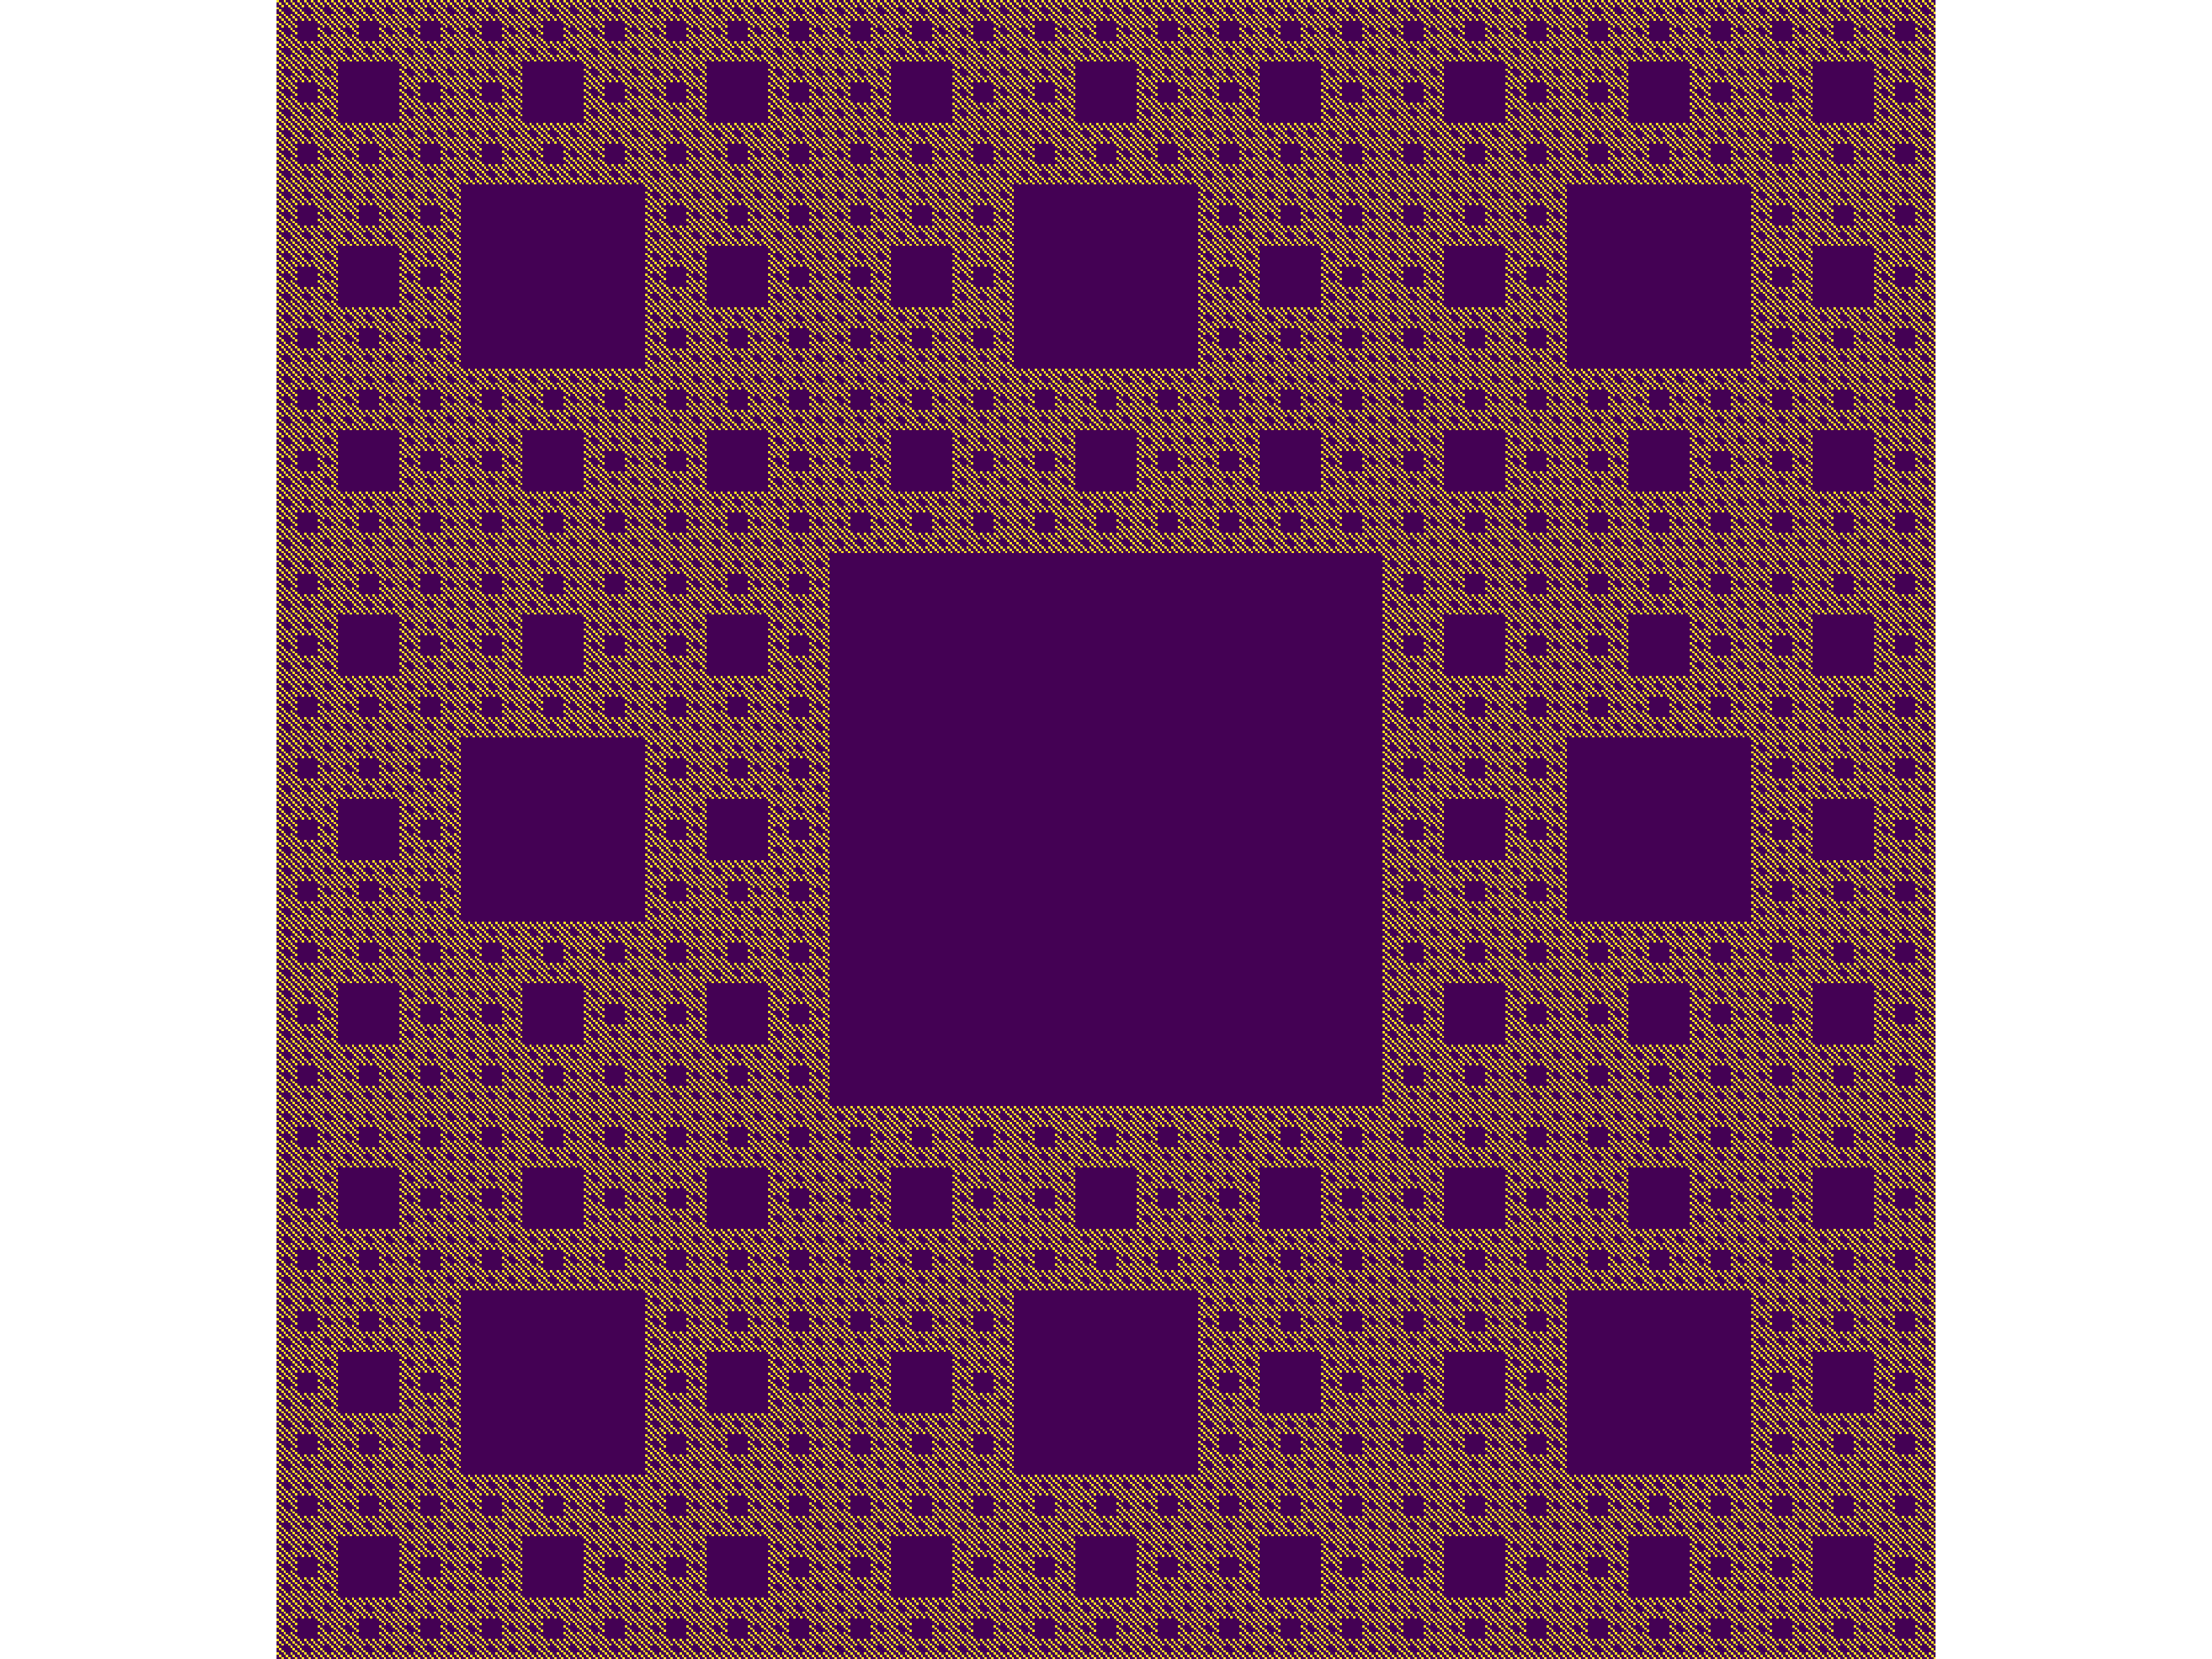
\includegraphics[width=9cm]{./media/sierpinsky_carpet.png}
\caption{\label{square-carpet}Sierpinksi's Carpet}
\end{figure}}

\begin{figure}[htbp]
\centering
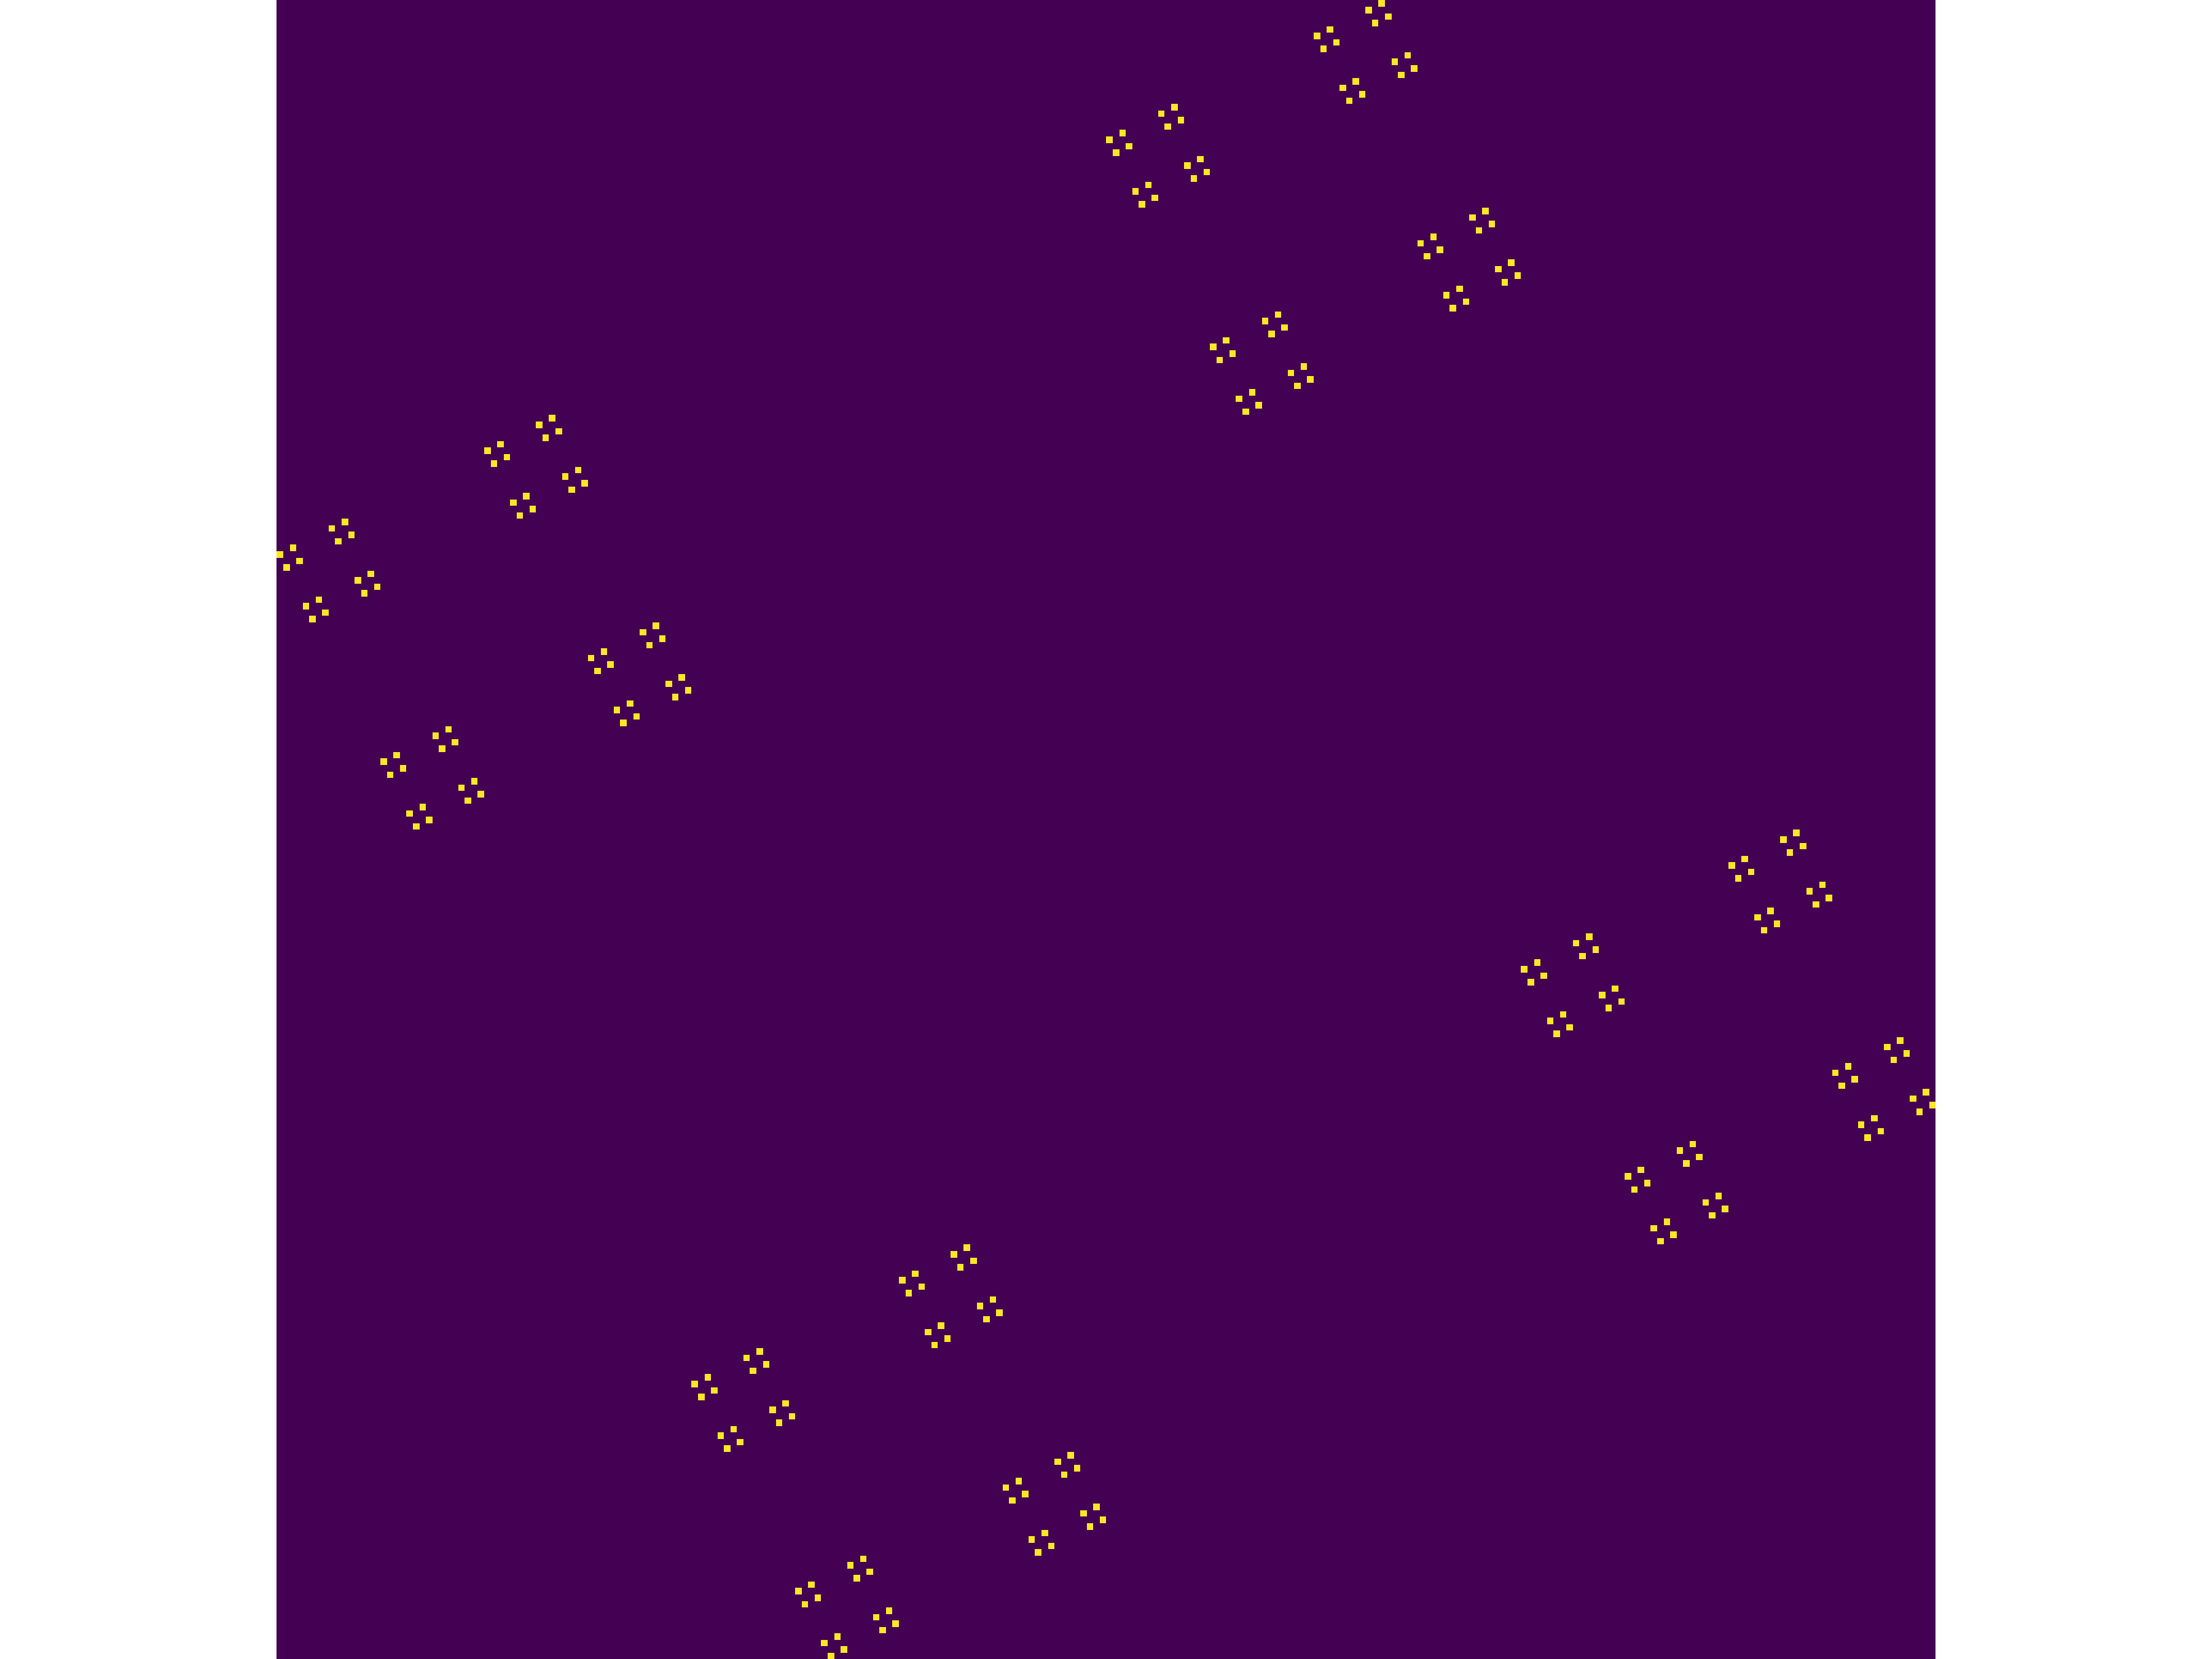
\includegraphics[width=9cm]{media/Cantor_Dust_gen.png}
\caption{\label{cantor-dust}Cantor Dust}
\end{figure}

\paragraph{Triangle}
\label{sec:org702ba8a}
Producing the triangle was more difficult
\subparagraph{Chaos Game}
\label{sec:org4dd3353}
This would be more accurate than pascals because there would be know \textbf{bias} and the model would be more accurate    :

\begin{listing}[htbp]
\begin{minted}[]{r}
if (require("pacman")) {
    library(pacman)
  }else{
    install.packages("pacman")
    library(pacman)
  }
  pacman::p_load(tidyverse)


n <- 50000
df <- data.frame("xval"=1:n, "yval"=1:n)

x <- c(runif(1), runif(1))
A <- c(0, 0)
B <- c(1, 0)
C <- c(0.5, sin(pi/3))
points <- list()
points <- list(points, x)


for (i in 1:n) {
    dice = sample(1:3, 1)
    if (dice == 1) {
        x <- (x + A)/2
        df[i,] <- x
    } else if (dice == 2) {
        x <- (x + B)/2
        df[i,] <- x
    } else {
        x <- (x + C)/2
        df[i,] <- x
    }
}

# df

ggplot(df, aes(x = xval, y = yval)) +
    geom_point(size = 1, col = "cadet blue") +
    theme_classic()

\end{minted}
\caption{R code to construct Sierpinksi's triangle through the Choas Game concept.}
\end{listing}


\begin{center}
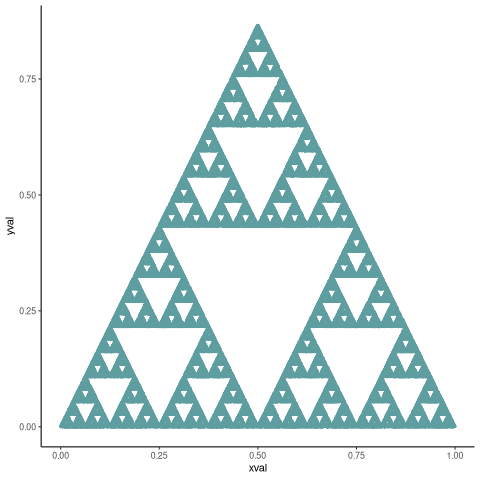
\includegraphics[width=.9\linewidth]{pascal-sierpinsky-chaos-game.png}
\end{center}

\subparagraph{Pascals Triange}
\label{sec:org80c58dd}

\begin{listing}[htbp]
\begin{minted}[]{julia}
function pascal(n)
    mat = [isodd(binomial(BigInt(j+i),BigInt(i))) for i in 0:n, j in 0:n]
    return mat
end
GR.imshow(pascal(999))
GR.savefig("../../Report/media/pascal-sierpinsky-triangle.png")

#------------------------------------------------------------
#-- Calculate Dimension -------------------------------------
#------------------------------------------------------------

mat2 = pascal(3000)
l2   = sum(mat2)
size2 = size(mat2)[1]
mat1 = pascal(2000)
l1   = sum(mat1)
size1 = size(mat1)[1]
log(l2/l1)/log(size2/size1)
# https://en.wikipedia.org/wiki/Sierpi%C5%84ski_triangle
log(3)/log(2)


\end{minted}
\caption{\label{pascal-triangle-sierpinski}Julia code demonstrating Sierpinksi's triangle}
\end{listing}

\begin{figure}[htbp]
\centering
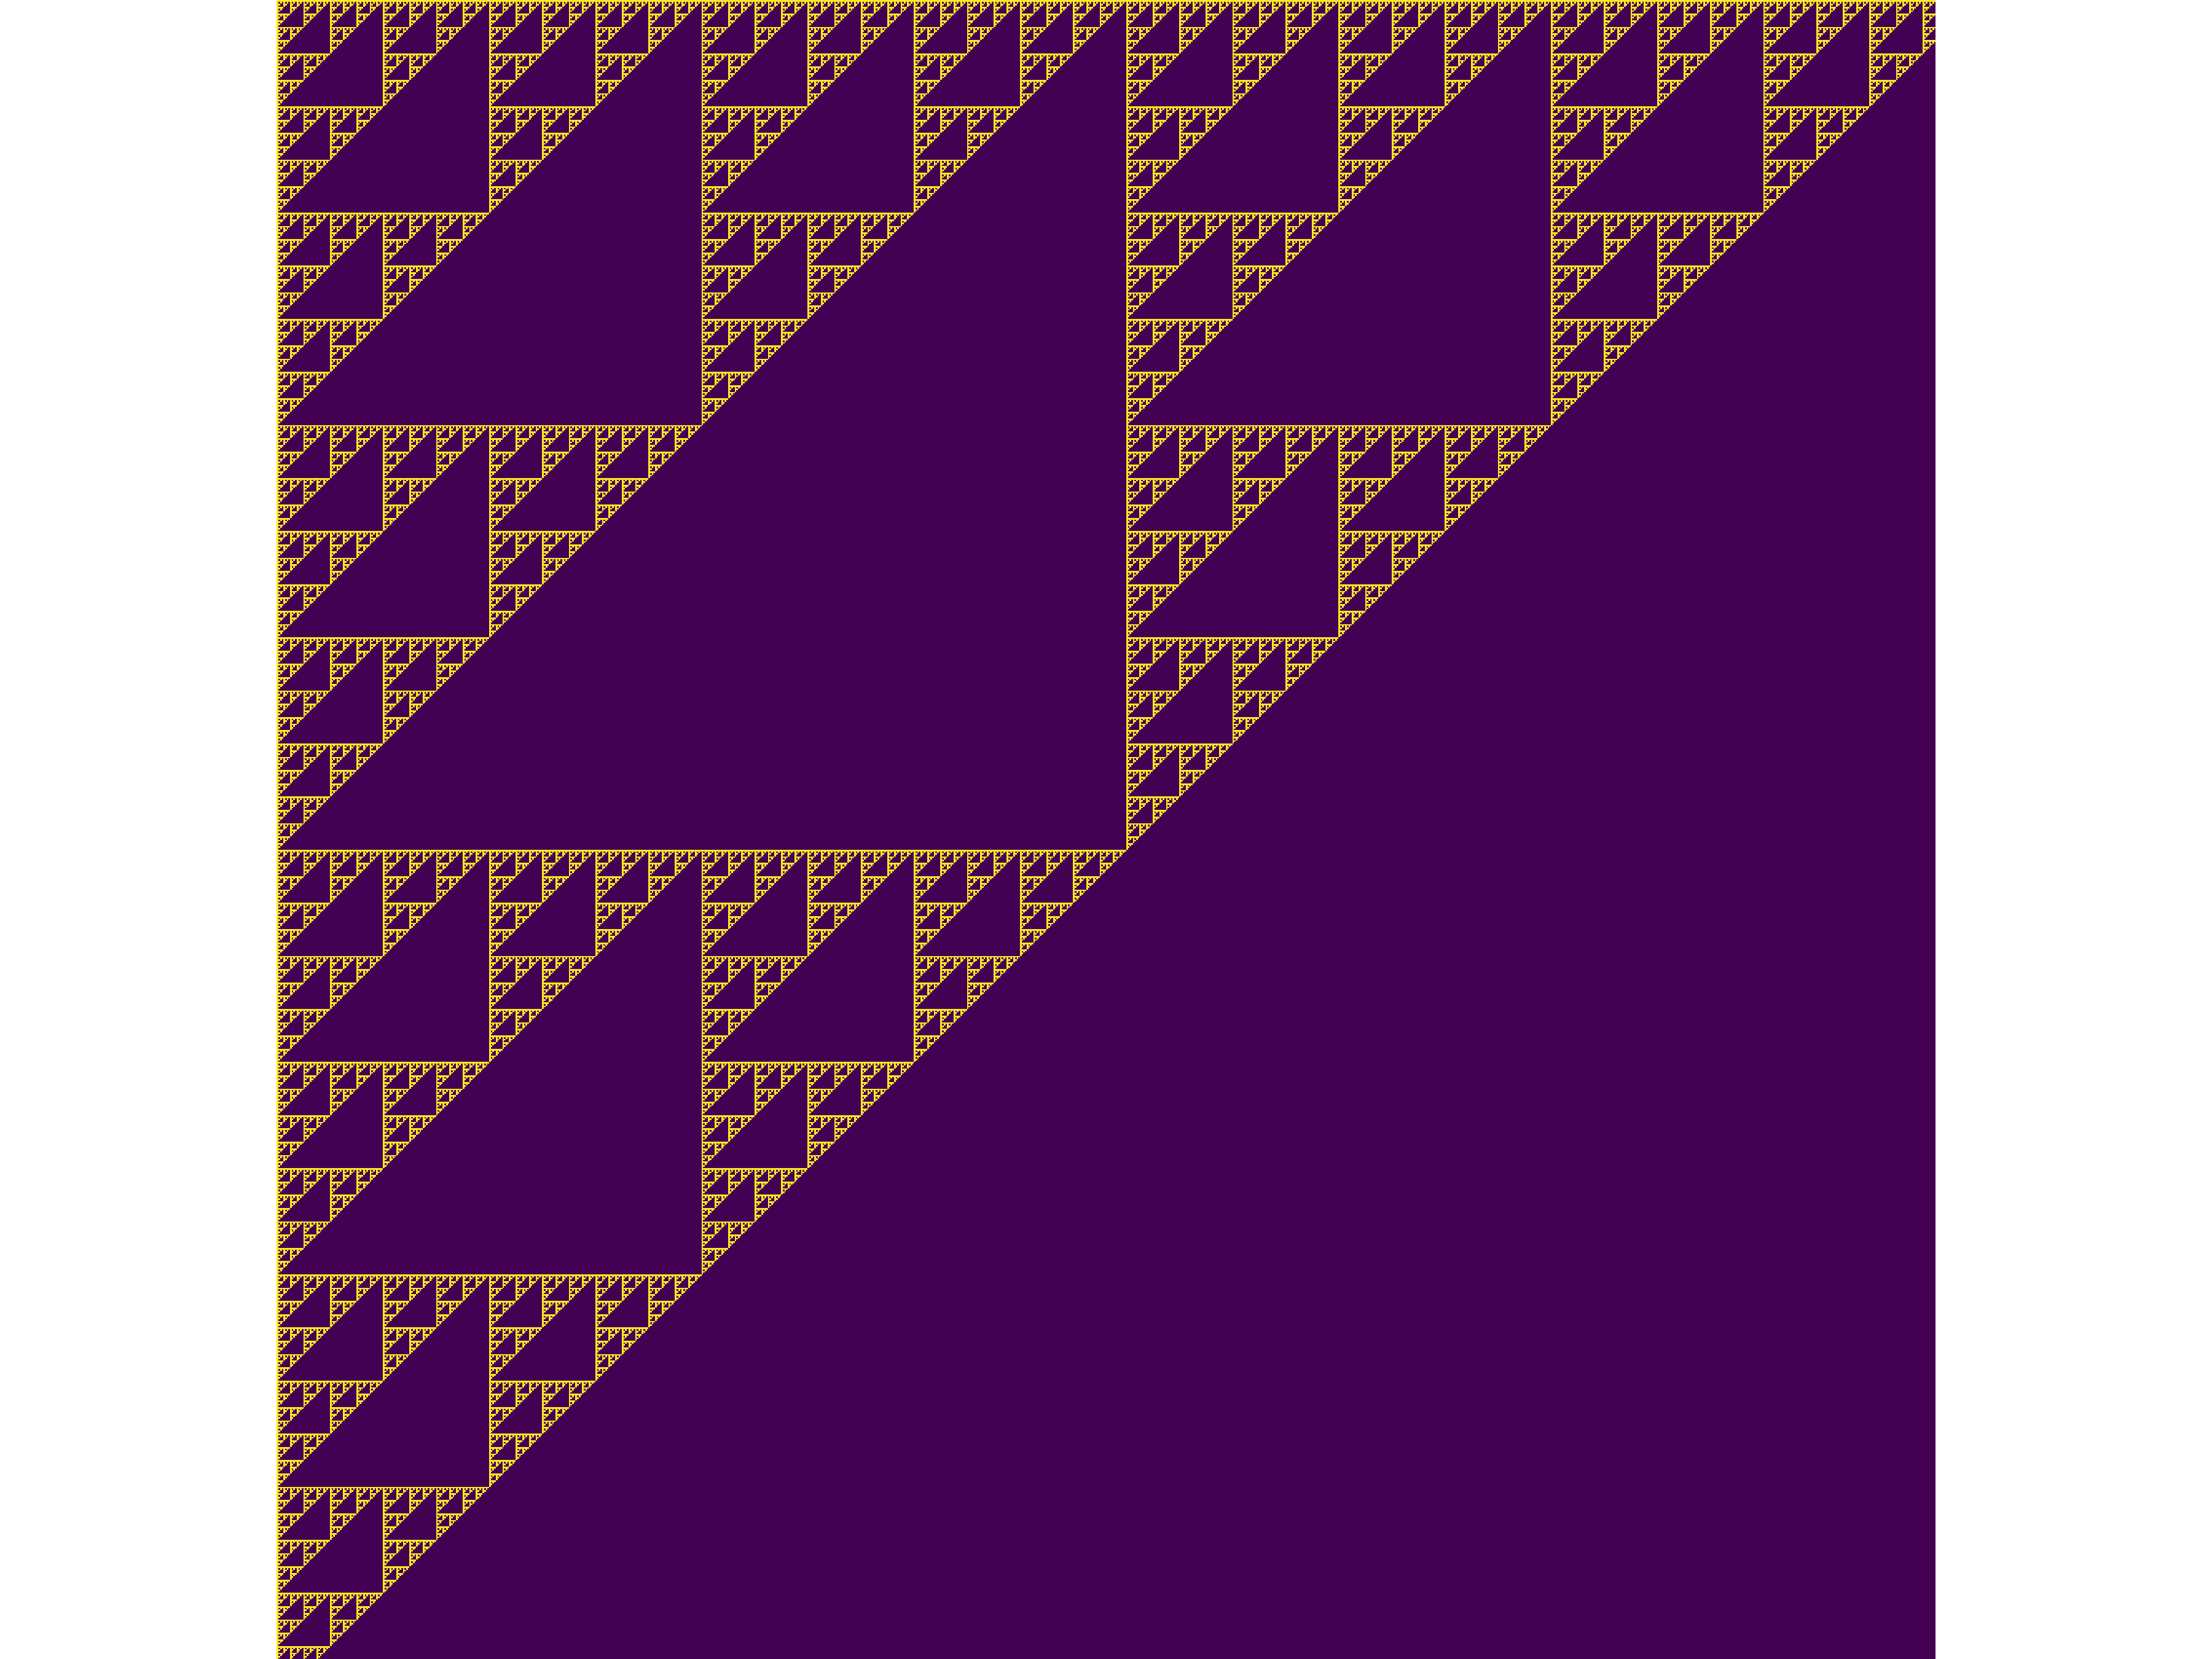
\includegraphics[width=9cm]{media/pascal-sierpinsky-triangle.png}
\caption{\label{fig:pascal-sierpinsky}TODO}
\end{figure}

\begin{enumerate}
\item Motivation
\label{sec:org8e5aac5}
Over many centuries, mathematicians have been able to produce a range of patterns from Pascal's triangle. One of which is relevant to the emergence of Sierpinski's triangle. To construct Pascal's triangle it begins with a 1 in the \(0^{th}\) (top) row, then each row underneath is made up of the sum of the numbers directly above it, see figure \ref{fig:pascal-triangle}. Alternatively, the \(n^{th}\) row and \(k^{th}\) column can be written in combinatorics form, \(\binom{n}{k} = \binom{n-1}{k-1} + \binom{n-1}{k}\).

\begin{figure}[htbp]
\centering
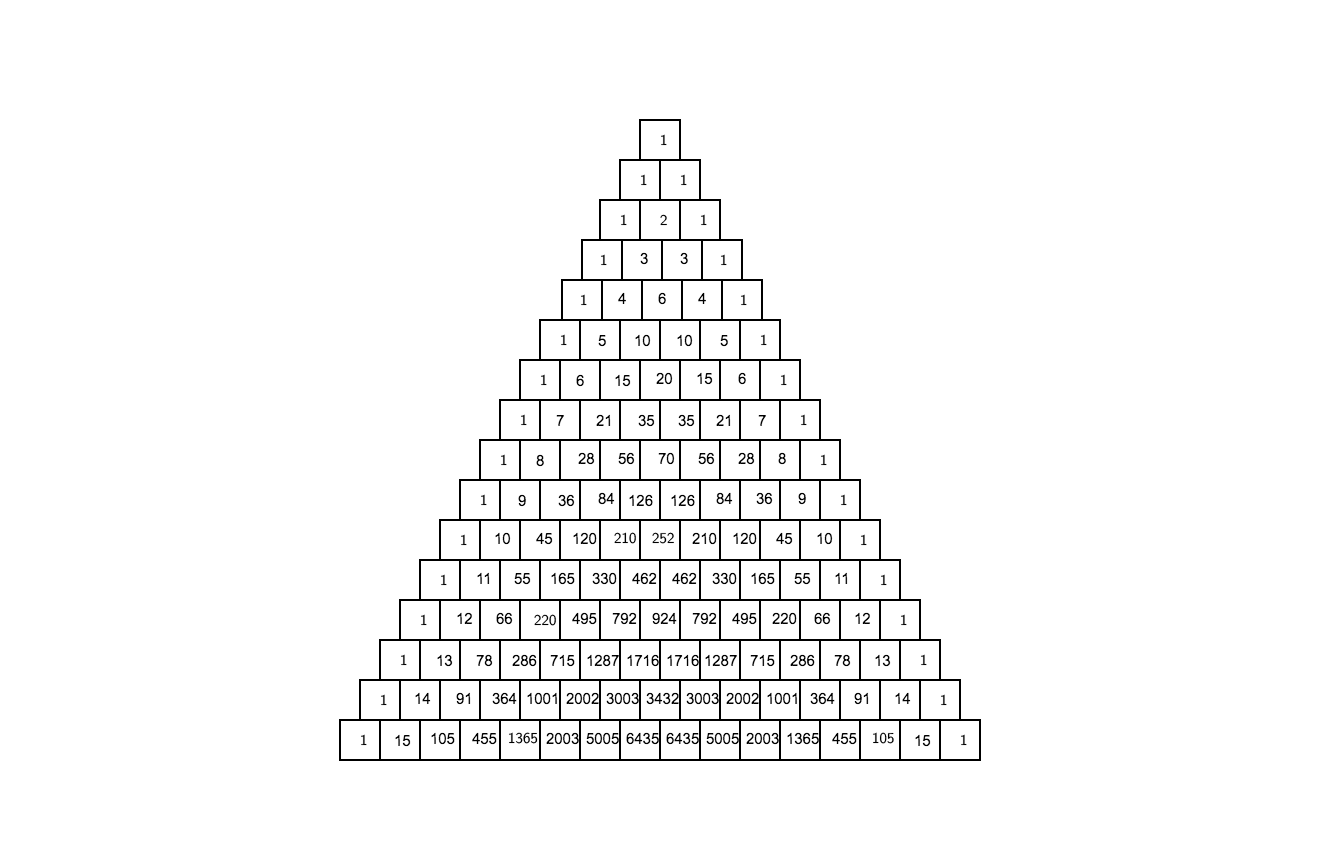
\includegraphics[width=.9\linewidth]{media/tikz/pascals-triangle.png}
\caption{\label{fig:pascal-triangle}Pascal's triangle}
\end{figure}

\item The connection
\label{sec:org2e007fd}
As mentioned before there is one pattern that produces the Sierpinski triangle, namely highlighting all odd numbers in Pascal's triangle. This is equivalent to considering all the numbers in the triangle modulo 2, shown in figure \ref{fig:pascal-sierpinski-tri}.

\begin{figure}[htbp]
\centering
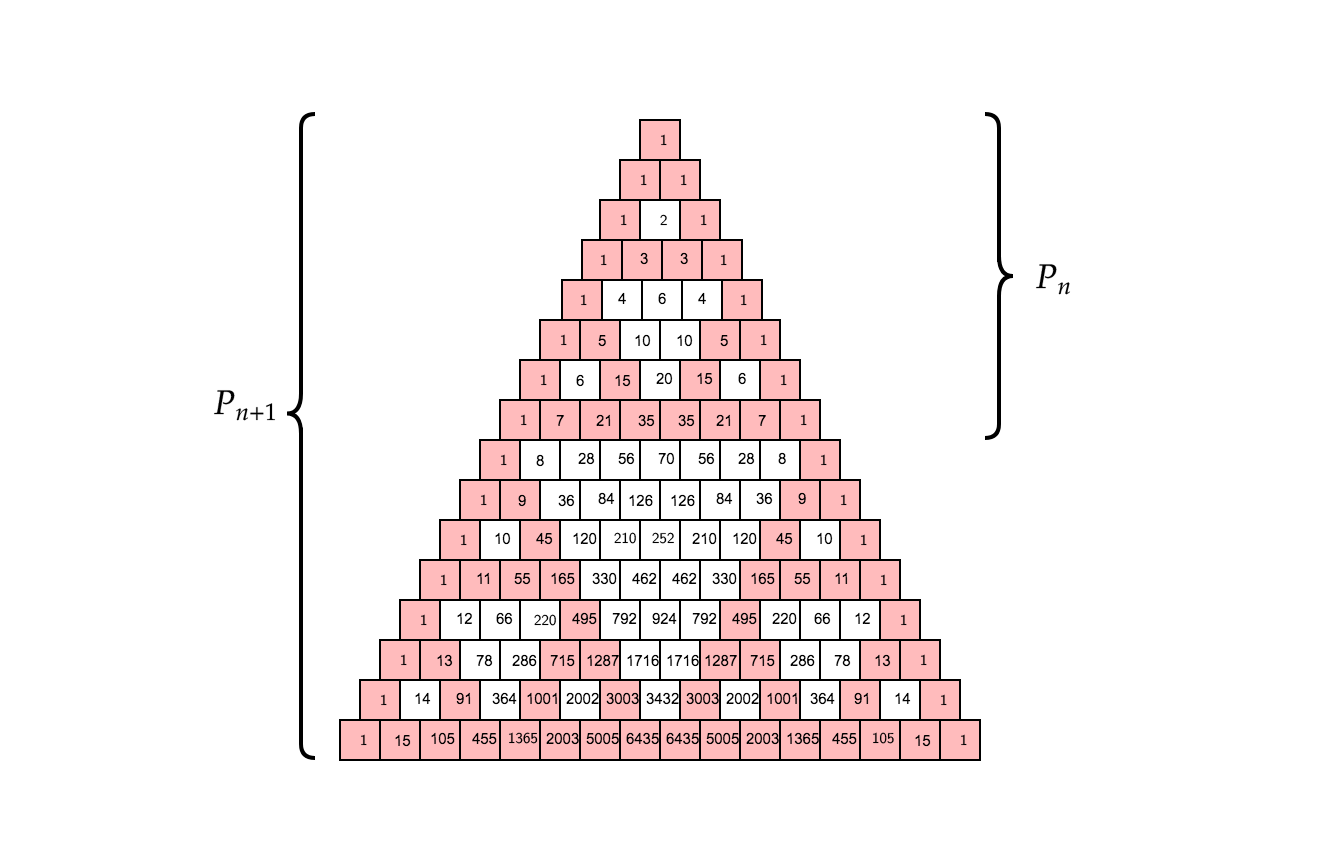
\includegraphics[width=9cm]{media/tikz/pascal-sierpinski-tri.png}
\label{fig:pascal-sierpinski-tri}
\end{figure}

\begin{figure}[htbp]
\centering
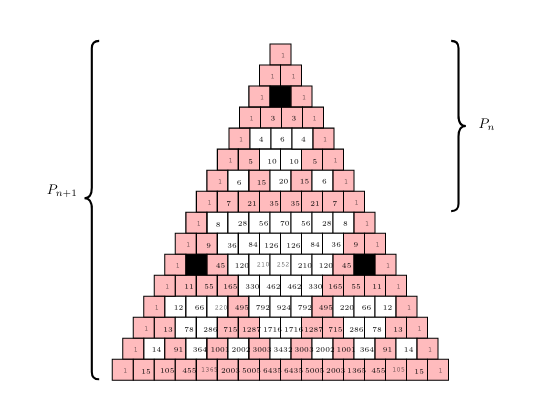
\includegraphics[width=9cm]{media/tikz/row-column-pascal.png}
\caption{\label{fig:row-column-pascal}The black squares represent one example of a position on Pascal's triangle that are equivalent modulo 2}
\end{figure}

In figure \ref{fig:pascal-sierpinski-tri}, we can observe that all the highlighted odd numbers begin to form the Sierpinski triangle. Note that this is not the complete Sierpinski's triangle, that would require an infinite number of iterations. Now, we also notice that there are three identical Sierpinski triangles within the larger triangle, each containing the same value modulo 2, at each corresponding row and column.

To prove this, we need to split the triangle into two parts, \(P_{n}\) denoting the first \(2^{n}\) rows, i.e. the top ``Sierpinski triangle'' in figure \ref{fig:pascal-sierpinski-tri} and \(P_{n+1}\) representing the entire triangle. We must show that any chosen square in \(P_{n}\) is equal to the corresponding row and column in the lower two triangles of \(P_{n+1}\), shown in figure \ref{fig:row-column-pascal}. This requires an identity that allows us to work with combinations in modulo 2, namely Lucas' Theorem.

\textbf{Lucas' Theorem}
Let \(n,k \ge 0\) and for some prime \(p\), we get:
\begin{equation}
\binom{n}{k} = \prod_{i=0}^{m} \binom{n_i}{k_i} \quad (\text{mod}~p)
\end{equation}
where,
\begin{align*}
n &= n_{m}p^{m}+n_{m-1}p^{m-1}+\cdots + n_{1}p+n_{0},\\
k &= k_{m}p^{m}+k_{m-1}p^{m-1}+\cdots + k_{1}p+k_{0}\\
\end{align*}
are the expansions in radix \(p\) \footnote{Radix refers to a numerical system which uses some number of digits. Since we are working in modulo 2 for Pascal's triangle, we are only concerned with the numbers \(0\) or \(1\), i.e. a radix 2 or a binary numeric system.}. This uses the convention that \(\binom{n}{k} = 0\) if \(k < n\)

Take some arbitrary row \(r\) and column \(c\) in the triangle \(P_{n}\). If we add \(2^{n}\) rows to \(r\), we will reach the equivalent row and column in the lower left triangle of \(P_{n+1}\), since there are \(2^{n}\) rows in \(P_{n}\). In the same way, if we add \(2^{n}\) columns to \(c\) we reach the equivalent row and column in the lower right triangle of \(P_{n+1}\), leaving us with:

\begin{align*}
\text{Top Triangle:} \quad &\binom{r}{c} \label{eq:top} \\
\text{Bottom-left Triangle:}\quad &\binom{r + 2^n}{c} \label{eq:bottom-left} \\
\text{Bottom-right Triangle :}\quad &\binom{r + 2^n}{c + 2^n} \label{eq:bottom-right}
\end{align*}

Using Lucas' theorem, we can prove that the above statments are equivalent.

We can rewrite \(r\) and \(c\) in base 2 notation as follows:
\begin{align*}
r=r_{i}2^{i}+r_{i-1}2^{i-1}+\cdots + r_{1}2+r_{0}= \left[r_{i}r_{i-1}\cdots r_{1}r_{0}\right]_2\\
c=c_{i}2^{i}+c_{i-1}2^{i-1}+\cdots +c_{1}2+c_{0}=\left[c_{i}c_{i-1}\cdots c_{1}c_{0}\right]_2\\
\end{align*}

\begin{align*}
\binom{2^n + r}{c}~(\text{mod}~2) &= \binom{1r_{i-1}r_{i-2} \cdots r_{0}}{0c_{i-1}c_{i-2} \cdots c_{0}} \quad (\text{mod} 2)\\
&= \binom{1}{0}\binom{r_{i-1}}{c_{i-1}}\binom{r_{i-2}}{c_{i-2}} \cdots \binom{r_0}{c_0} \quad (\text{mod} 2)\\
&=\binom{r_{i-1}}{c_{i-1}}\binom{r_{i-2}}{c_{i-2}} \cdots \binom{r_0}{c_0} \quad (\text{mod} 2)\\
&= \binom{r}{c} \quad (\text{mod} 2)
\end{align*}

\begin{align*}
\binom{2^n + r}{2^n + c}~(\text{mod}~2) &= \binom{1r_{i-1}r_{i-2} \cdots r_{0}}{1c_{i-1}c_{i-2} \cdots c_{0}} \quad (\text{mod} 2)\\
&= \binom{1}{1}\binom{r_{i-1}}{c_{i-1}}\binom{r_{i-2}}{c_{i-2}} \cdots \binom{r_0}{c_0} \quad (\text{mod} 2)\\
&=\binom{r_{i-1}}{c_{i-1}}\binom{r_{i-2}}{c_{i-2}} \cdots \binom{r_0}{c_0} \quad (\text{mod} 2)\\
&= \binom{r}{c} \quad (\text{mod} 2)
\end{align*}

Thus, \(\binom{r}{c} = \binom{2^n + r}{c} = \binom{2^n + r}{2^n + c} \quad (\text{mod} 2)\), which concludes the proof

\item Comment on the dimension lining up
\label{sec:org0901f02}
Using the box-counting method, we can evaluate the dimension of Sierpinski's triangle.
\item FIx the value
\label{sec:org19d343d}

\begin{verbatim}

julia> log(l2/l1)/log(size2/size1)
2.082583161459976

julia> # https://en.wikipedia.org/wiki/Sierpi%C5%84ski_triangle
       log(3)/log(2)
1.5849625007211563

\end{verbatim}
\end{enumerate}

\subsubsection{Turtle}
\label{sec:orgdd67fb7}
Matrices can't explain all patterns, Turtles are useful
\begin{listing}[htbp]
\begin{minted}[]{julia}
using Shapefile
using Luxor
using Pkg


#------------------------------------------------------------
#-- Dragon Curve -------------------------------------
#------------------------------------------------------------


function snowflake(length, level, ♘, s)
    scale(s)
    if level == 0
        Forward(♘, 100)
        Turn(♘, -90)
        Rotate(90)
#        Rectangle(♘, length, length)
        return
    end
    length = length/9
    snowflake(length, level-1, ♘)
    Turn(♘, -60)
    snowflake(length, level-1, ♘)
    Turn(♘, 2*60)
    snowflake(length, level-1, ♘)
    Turn(♘, -180/3)
    snowflake(length, level-1, ♘)
end
@png begin
    ♘ = Turtle()
    Pencolor(♘, 1.0, 0.4, 0.2)
    Penup(♘)
    Turn(♘,180)
    Forward(♘, 200)
    Turn(♘,180)
    Pendown(♘)
    levels = 10
    snowflake(9^(levels), levels, ♘, 1)
end 800 800 "./snowFlat600.png"


#------------------------------------------------------------
#-- Flat Snowflake ----------------------------------
#------------------------------------------------------------


function snowflake(length, level, ♘, s)
    scale(s)
    if level == 0
        Forward(♘, length)
#        Rectangle(♘, length, length)
        return
    end
    length = length/9
    snowflake(length, level-1, ♘)
    Turn(♘, -60)
    snowflake(length, level-1, ♘)
    Turn(♘, 2*60)
    snowflake(length, level-1, ♘)
    Turn(♘, -180/3)
    snowflake(length, level-1, ♘)
end
@png begin
    ♘ = Turtle()
    Pencolor(♘, 1.0, 0.4, 0.2)
    Penup(♘)
    Turn(♘,180)
    Forward(♘, 200)
    Turn(♘,180)
    Pendown(♘)
    levels = 10
    snowflake(9^(levels), levels, ♘, 1)
end 800 800 "/tmp/snowFlat600.png"


#------------------------------------------------------------
#--- Round Snowflake Working ---------------------------------
#------------------------------------------------------------

function snowflake(length, level, ♘)
if level == 0
#    Forward(♘, length)
    Circle(♘, 1)
    return
end
length = length/9
snowflake(length, level-1, ♘)
Turn(♘, -60)
snowflake(length, level-1, ♘)
Turn(♘, 2*60)
snowflake(length, level-1, ♘)
Turn(♘, -60)
snowflake(length, level-1, ♘)
end
♘ = Turtle()
@svg begin
for i in 1:3
    levels = 9
    snowflake(8^(levels-1), levels, ♘)
    Turn(♘, 120)
end
end 2000 2000 "/tmp/snowCurve.svg"



0 "/tmp/snowCurve.png"

# The starting length must be such that the final length = 1 pixel
# this depends on the levels
# The levels must hence be fit to the resolution such that
# the only variable is the resolution.
# There is only two variables levels and resolution
# length depends on the levels and for a perfect snowflake
# the levels depends on the resolution.


using Images, TestImages, Colors, ImageMagick
# Load Image Back in
img = load("/tmp/snowCurve.png")
# Convert to Grayscale so only 2D
imgg = Gray.(img)
# convert to Matrix
mat = convert(Array{Float64}, imgg)

# 1 is white
    # so make all 1s 0 and everything else 1

for i in 1:size(mat)[1]
    for j in 1:size(mat)[2]
        if mat[i, j]==1
            mat[i,j]=0
        else
            mat[i,j]=1
        end
    end
end


sum(mat)

using GR
GR.imshow(mat)
mat

mat2 = selfRep(fill(1, 1, 1), 1000)
l2   = sum(mat2)
size2 = size(mat2)[1]
mat1 = selfRep(fill(1, 1, 1), 500)
l1   = sum(mat1)
size1 = size(mat1)[1]
log(l2/l1)/log(size2/size1)
# https://en.wikipedia.org/wiki/Vicsek_fractal#Construction
log(5)/log(3)

#------------------------------------------------------------
#--- Dragon -------------------------------------------------
#------------------------------------------------------------
function dragon(♘, order, length)
    print(" ") # Don't remove this or code breaks, I don't know why?
    Turn(♘, order*45)
    dragon_iterate(♘, order, length, 1)
end
function dragon_iterate(♘, order, length, sign)
    if order==0
        Forward(♘, length)
    else
        rootHalf = sqrt(0.5)
        dragon_iterate(♘, order -1, length*rootHalf, 1)
        Turn(♘, sign * -90)
        dragon_iterate(♘, order -1, length*rootHalf, -1)
    end
end
;mkdir /tmp/dragon
@png begin
    ♘ = Turtle()
    Turn(♘, 180)
    Penup(♘)
    Forward(♘, 200)
    Pendown(♘)
    Turn(♘, 180)
    dragon(♘, 15, 400)
end 1000 1000

using Images, TestImages, Colors, ImageMagick
# Load Image Back in
img = load("/tmp/dragon.png")
# Convert to Grayscale so only 2D
imgg = Gray.(img)
# convert to Matrix
mat = convert(Array{Float64}, imgg)

# 1 is white
    # so make all 1s 0 and everything else 1

for i in 1:size(mat)[1]
    for j in 1:size(mat)[2]
        if mat[i, j]==1
            mat[i,j]=0
        else
            mat[i,j]=1
        end
    end
end


\end{minted}
\caption{\label{turtles-all}This generates a dragon and a koch}
\end{listing}
\paragraph{Dragon Curve}
\label{sec:org4cd762a}

\begin{figure}[htbp]
\centering
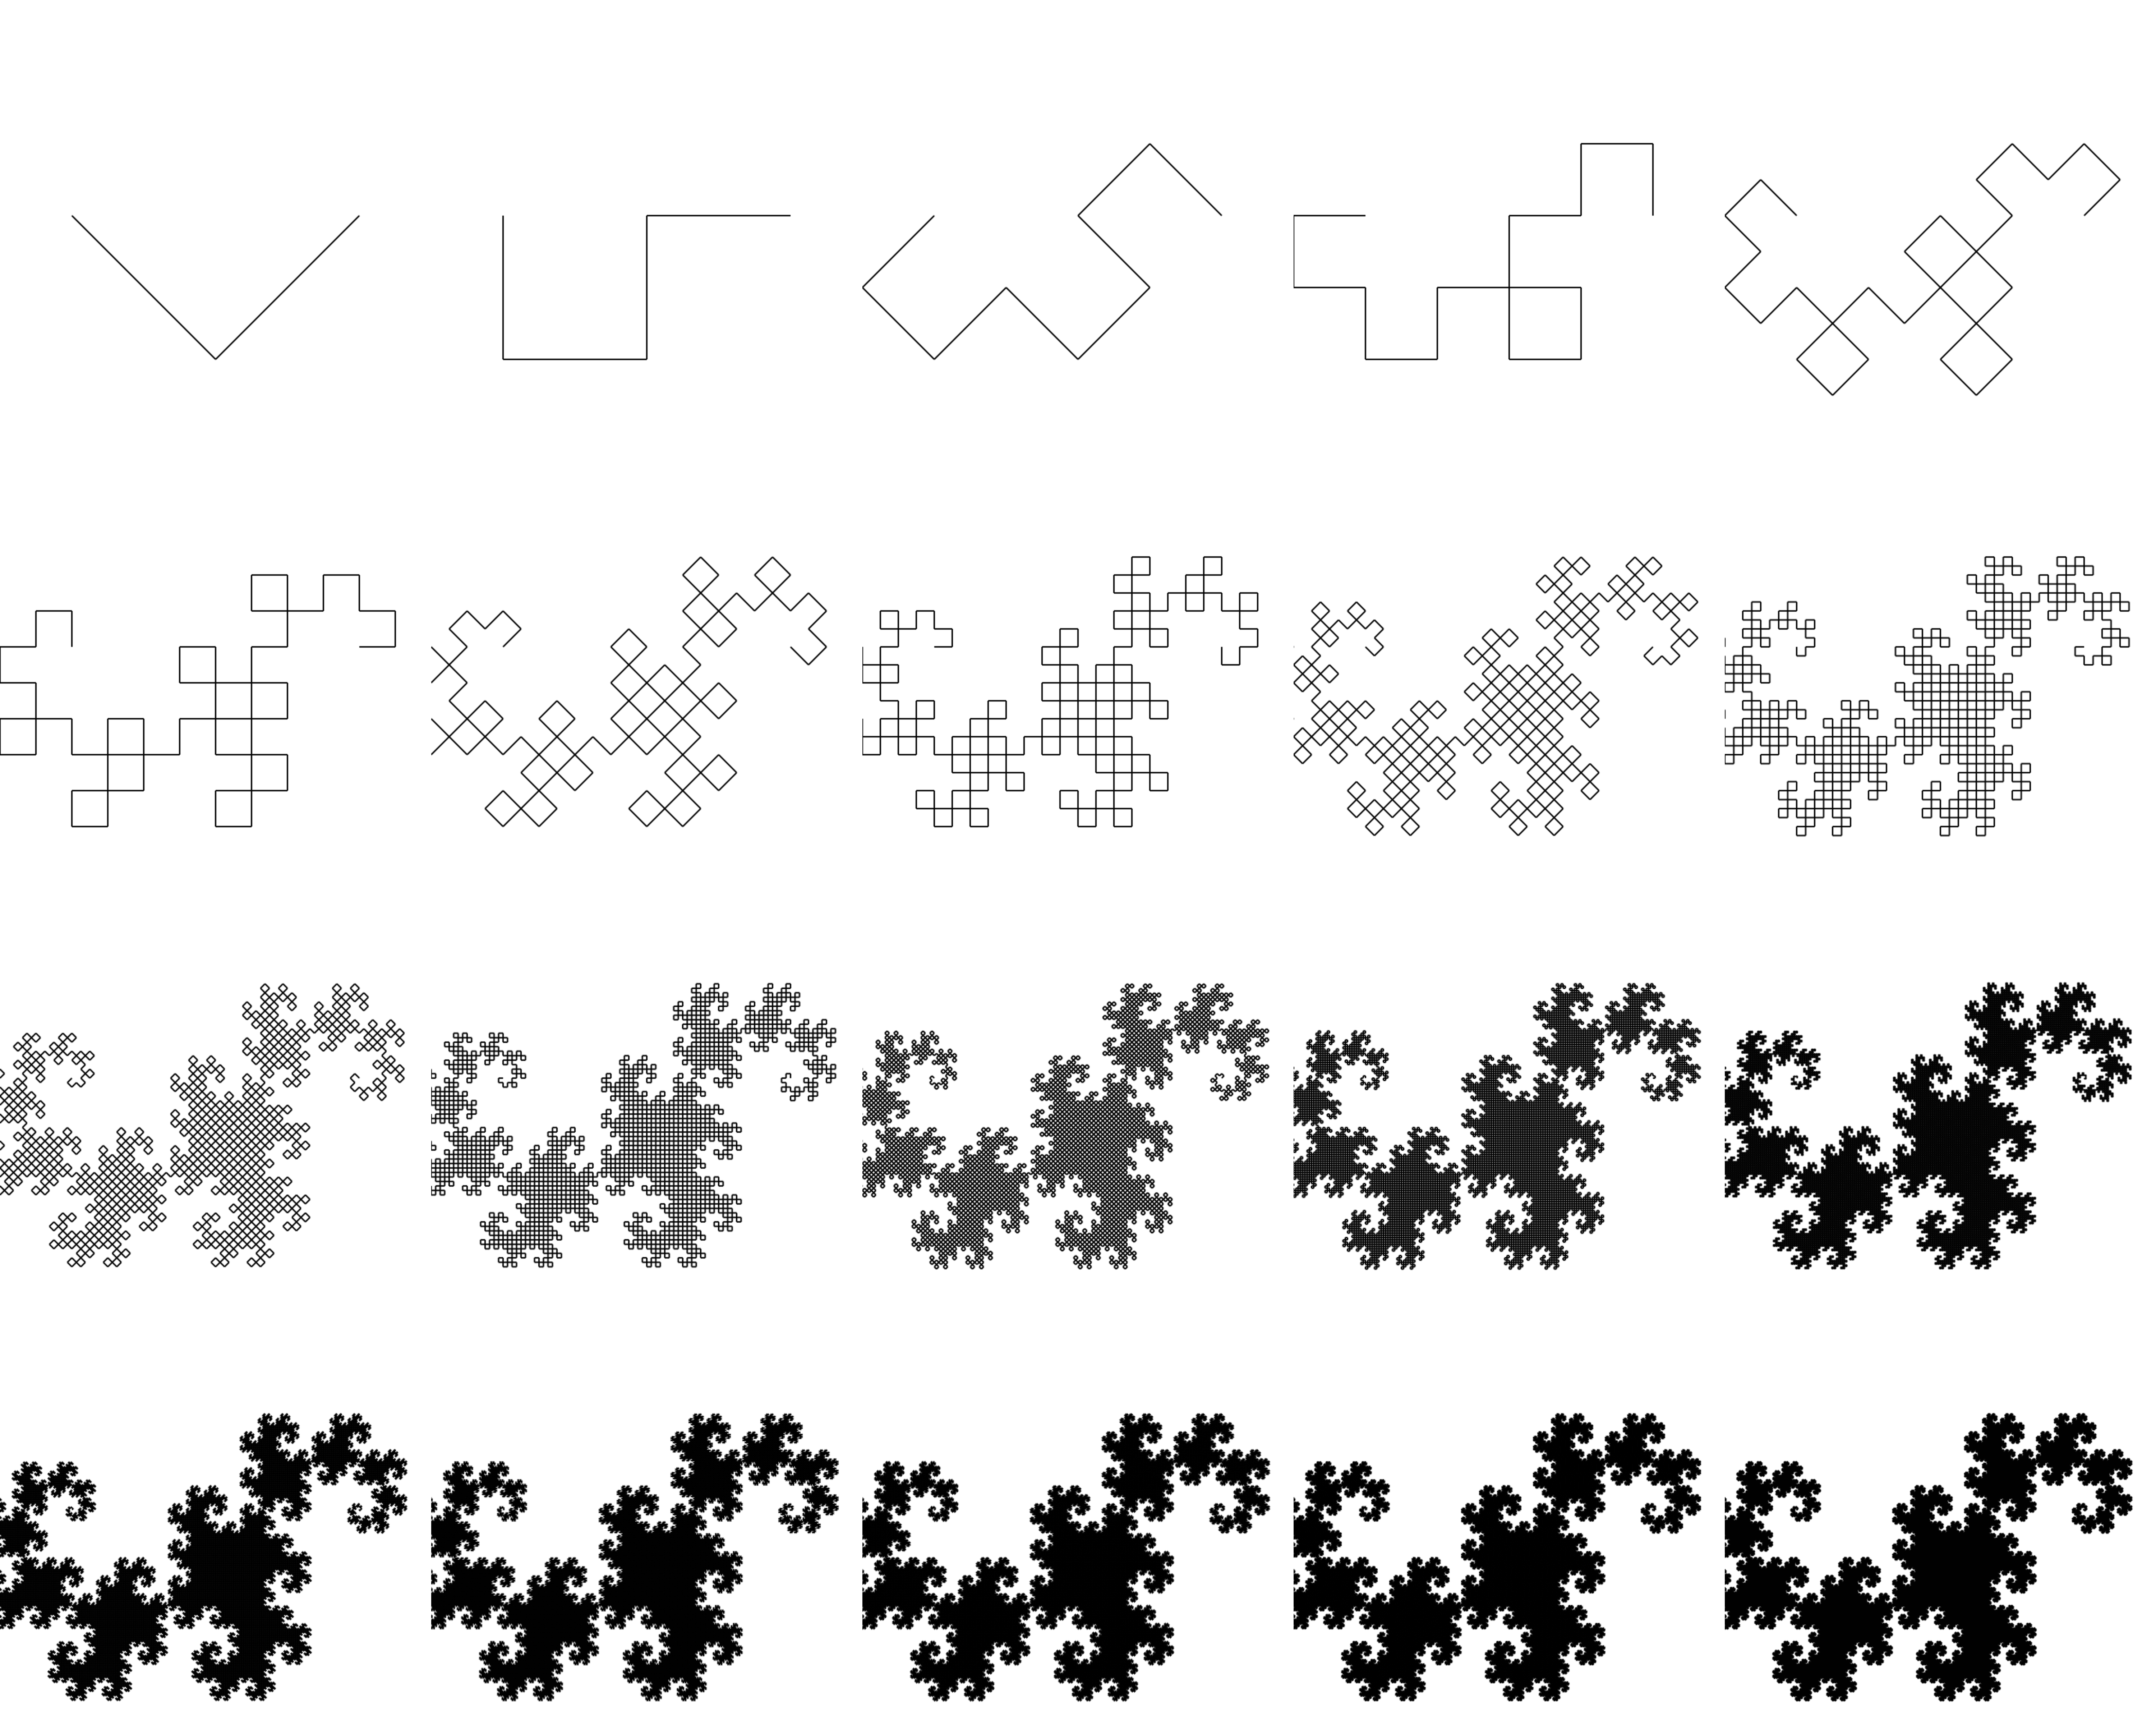
\includegraphics[width=9cm]{../Problems/Chaos/Spirals/dragon.png}
\caption{\label{dragon-turtle}TODO}
\end{figure}


\paragraph{Koch Snowflake}
\label{sec:orgfbd5e1d}
\begin{figure}[htbp]
\centering
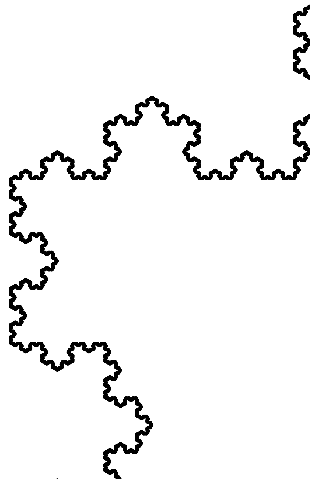
\includegraphics[width=9cm]{../Problems/Chaos/Spirals/snowCurve.png}
\caption{\label{dragon-turtle}TODO}
\end{figure}

\subsection{Fractal Dimensions}
\label{sec:orge834686}
\subsubsection{Calculating the Dimension of Julia Set}
\label{sec:orge3852f0}
It converges too slowly
The Julia set (discussed in section ) can be solved by \ldots{}

explain the code a little bit here

as shown in listing

A value on the complex plane can be associated with the julia set by iterating
that value against a function of the form \(z \rightarrow z^{2} + \alpha + i
\beta\) and measureing whether or not that value diverges or converges. This process is demonstrated in listing \ref{jsetDivFunc}.

By associating each value on the complex plane with an element of a matrix an image of this pattern may be produced, see for example figure RABBIT

\begin{listing}[htbp]
\begin{minted}[]{julia}
#!/bin/julia
function juliaSet(z, num, my_func, boolQ=true)
    count = 1
    # Iterate num times
    while count ≤ num
        # check for divergence
        if real(z)^2+imag(z)^2 > 2^2
            if(boolQ) return 0 else return Int(count) end
        end
        #iterate z
        z = my_func(z) # + z
        count=count+1
    end
        #if z hasn't diverged by the end
    if(boolQ) return 1 else return Int(count) end
end
\end{minted}
\caption{\label{jsetDivFunc}Function that returns how many iterations of a function of is necessary for a complex value to diverge, the julia set is concerned with the function \(z \rightarrow z^{2} + \alpha + i \beta\)}
\end{listing}


So I run the code shown in listing \ref{dimensions-julia-set} which calls a file \texttt{./Julia-Set-Dimensions-functions.jl} which is shown in listing \ref{functions-julia-set} which returs the values shown in table \ref{table-of-values}.

\begin{minted}[]{julia}
@time include("./Julia-Set-Dimensions-functions.jl")

############################################################
#### Investigate Plot #######################################
############################################################

f(z) = z^2 -1

test_mat = make_picture(800,800, z -> z^2 + 0.37-0.2*im)
test_mat = make_picture(800,800, z -> z^2 + -0.123+0.745*im)
test_mat = make_picture(800,800, f)
GR.imshow(test_mat) # PyPlot uses interpolation = "None"


test_mat = outline(test_mat)
GR.imshow(test_mat) # PyPlot uses interpolation = "None"
# GR.savefig("/home/ryan/Dropbox/Studies/2020Spring/QuantProject/Current/Python-Quant/Problems/fractal-dimensions/media/outline-Julia-set.png")

## Return the perimeter
sum(test_mat)



mat2 = outline(make_picture(9000,9000, f))
l2   = sum(mat2)
size2 = size(mat2)[1]
mat1 = outline(make_picture(10000,10000, f))
l1   = sum(mat1)
size1 = size(mat1)[1]
log(l2/l1)/log(size2/size1)
# https://en.wikipedia.org/wiki/Vicsek_fractal#Construction
# 1.3934 Douady Rabbit
#





using CSV

@time data=scaleAndMeasure(9000, 10000 , 4, f)
# CSV.read("./julia-set-dimensions.csv", data)
# data = CSV.read("./julia-set-dimensions.csv")
data.scale = [log(i) for i in data.scale]
data.mass  = [log(i) for i in data.mass]
mod   = lm(@formula(mass ~ scale), data)
p = Gadfly.plot(data, x=:scale, y=:mass, Geom.point)

print("the slope is $(round(coef(mod)[2], sigdigits=4))")
print(mod)
print("\n")
return mod

a = SharedArray{Float64}(10)
@distributed for i = 1:10
    a[i] = i
end

# import Gadfly
#
# iris = dataset("datasets", "iris")
# p = Gadfly.plot(iris, x=:SepalLength, y=:SepalWidth, Geom.point);
# img = SVG("iris_plot.svg")
# draw(img, p)


# The trailing `;` supresses output, equivalently:



## Other Fractals to look at for this maybe?
  # GR.imshow(test_mat) # PyPlot uses interpolation = "None"
  # GR.imshow(make_picture(500, 500, z -> z^2 + 0.37-0.2*im)) # PyPlot uses interpolation = "None"
  # GR.imshow(make_picture(500, 500, z -> z^2 + 0.38-0.2*im)) # PyPlot uses interpolation = "None"
  # GR.imshow(make_picture(500, 500, z -> z^2 + 0.39-0.2*im)) # PyPlot uses interpolation = "None"
\end{minted}

\begin{minted}[]{julia}
using GR
using DataFrames
using Gadfly
using GLM
using SharedArrays
using Distributed

############################################################
### Julia / MandelBrot Functions ###########################
############################################################

"""
# Julia Set
Returns how many iterations it takes for a value on the complex plane to diverge
under recursion. if `boolQ` is specified as true a 1/0 will be returned to
indicate divergence or convergence.

## Variables
- `z`
  - A value on the complex plane within the unit circle
- `num`
  - A number of iterations to perform before conceding that the value is not
    divergent.
- `my_func`
  - A function to perform on `z`, for a julia set the function will be of the
    form `z -> z^2 + a + im*b`
    - So for example the Douady Rabbit would be described by `z -> z^2 -0.123+0.745*im`
"""
function juliaSet(z, num, my_func, boolQ=true)
    count = 1
    # Define z1 as z
    z1 = z
    # Iterate num times
    while count ≤ num
        # check for divergence
        if real(z1)^2+imag(z1)^2 > 2^2
            if(boolQ) return 0 else return Int(count) end
        end
        #iterate z
        z1 = my_func(z1) # + z
        count=count+1
    end
        #if z hasn't diverged by the end
    if(boolQ) return 1 else return Int(count) end
end


"""
# Mandelbrot Set
Returns how many iterations it takes for a value on the complex plane to diverge
under recursion of \$z \\rightarrow z^2 + z_0\$.

Values that converge represent constants of the julia set that lead to a
connected set. (TODO: Have I got that Vice Versa?)


## Variables
- `z`
  - A value on the complex plane within the unit circle
- `num`
  - A number of iterations to perform before conceding that the value is not
    divergent.
- `boolQ`
  - `true` or `false` value indicating whether or not to return 1/0 values
    indicating divergence or convergence respecitvely or to return the number of
   iterations performed before conceding no divergence.
"""
function mandelbrot(z, num, boolQ = true)
    count = 1
    # Define z1 as z
    z1 = z
    # Iterate num times
    while count ≤ num
        # check for divergence
        if real(z1)^2+imag(z1)^2 > 2^2
            if(boolQ) return 0 else return Int(count) end
        end
        #iterate z
        z1 = z1^2 + z
        count=count+1
    end
        #if z hasn't diverged by the end
    return 1 # Int(num)
    if(boolQ) return 1 else return Int(count) end
end

function test(x, y)
    if(x<1) return x else return y end
end


############################################################
##### Build a Matrix Image #################################
############################################################

"""
# Make a Picture

This maps a function on the complex plane to a matrix where each element of the
matrix corresponds to a single value on the complex plane. The matrix can be
interpreted as a greyscale image.

Inside the function is a `zoom` parameter that can be modified for different
fractals, fur the julia and mandelbrot sets this shouldn't need to be adjusted.

The height and width should be interpreted as resolution of the image.

- `width`
  - width of the output matrix
- `height`
  - height of the output matrix
- `myfunc`
  - Complex Function to apply across the complex plane
"""
function make_picture(width, height, my_func)
    pic_mat = zeros(width, height)
    zoom = 0.3
    for j in 1:size(pic_mat)[2]
        for i in 1:size(pic_mat)[1]
            x = (j-width/2)/(width*zoom)
            y = (i-height/2)/(height*zoom)
            pic_mat[i,j] = juliaSet(x+y*im, 256, my_func)
        end
    end
    return pic_mat
end

############################################################
### Make the Outline ########################################
############################################################
# TODO this should be inside a function

"""
# Outline

Sets all elements with neighbours on all sides to 0.

- `mat`
  - A matrix
    - If this matrix is the convergent values corresponding to a julia set the
      output will be the outline, which is the definition of the julia set.
"""
function outline(mat)
    work_mat = copy(mat)
    for col in 2:(size(mat)[2]-1)
        for row in 2:(size(mat)[1]-1)
            ## Make the inside 0, we only want the outline
            neighbourhood = mat[row-1:row+1,col-1:col+1]
            if sum(neighbourhood) >= 9 # 9 squares
                work_mat[row,col] = 0
            end
        end
    end
    return work_mat
end


############################################################
###### Return many Scaled Values ###########################
############################################################



function scaleAndMeasure(min, max, n, func)
    # The scale is equivalent to the resolution, the initial resolution could be
    # set as 10, 93, 72 or 1, it's arbitrary (previously I had res and scale)
    # #TODO: Prove this

    scale = [Int(ceil(i)) for i in range(min, max, length=n) ]
    mass = pmap(s -> sum(outline(make_picture(Int(s), Int(s), func))) , scale)

    data = DataFrame(scale = scale, mass = mass)
    return data
end

\end{minted}

This returns the Values:

\begin{table}[htbp]
\centering
\begin{tabular}{rr}
scale & mass\\
\hline
500 & 4834.0\\
563 & 5754.0\\
625 & 6640.0\\
688 & 7584.0\\
750 & 8418.0\\
813 & 9550.0\\
875 & 10554.0\\
938 & 11710.0\\
1000 & 12744.0\\
\end{tabular}
\caption{\label{table-of-values}TODO}

\end{table}
\paragraph{Using Linear Regression}
\label{linear-reg-julia}
\begin{itemize}
\item Avoiding \texttt{Abs} is twice as fast
\item Column wise is faster in fortran/julia/R slower in C/Python
We have no evidence to show that the dimension will be stable, this is good for coastlines and stuff.
\end{itemize}

This approach is layed out in \cite[p. 30]{vicsekFractalGrowthPhenomena1992}.
\subparagraph{Performance}
\label{sec:org960d528}
\begin{itemize}
\item Switching from \texttt{abs()} to sqaured help
\item Taking advantage of multi core processing in loops

\item \href{https://stackoverflow.com/a/55704326/12843551}{pmap was chosen because} it scales better for expensive jobs.

Comparison
\end{itemize}
\begin{minted}[]{julia}
function tme()
    start = time()
    data = scaleAndMeasure(900, 1000, 9)
    length = time() - start
    print(length, "\n")
    return length
end
times = [tme() for i in 1:10 ]
\end{minted}

\begin{center}
\begin{tabular}{lr}
Function & Mean Time\\
\texttt{pmap} & 2.2825\\
\end{tabular}

\end{center}
\section{Connecting Fractals to Natural Processes}
\label{my-fractal}
My fractal really shows many unique patterns

If it is scaled by \(\varphi\) then the boxes increase two fold.

We know the dimension will be constant because the figure is self similar, so we have:

\[
\mathrm{dim} (\mathtt{my\_fractal}) = \log_{\varphi}=\frac{\log \varphi}{\log 2}
\]
\subsection{Graphics}
\label{sec:org9276983}

\begin{figure}[htbp]
\centering
\includesvg[width=9cm]{../Problems/fractal-dimensions/scale-of-my-fractal}
\caption{\label{My-Frac-GR}TODO}
\end{figure}

\begin{figure}[htbp]
\centering
\includesvg[width=9cm]{../Problems/fractal-dimensions/my-self-rep-frac}
\caption{\label{My-Frac-GR}TODO}
\end{figure}

\begin{figure}[htbp]
\centering
\includesvg[width=9cm]{../Problems/fractal-dimensions/golden-angle-diagram}
\caption{\label{My-Frac-GR}TODO}
\end{figure}

\begin{figure}[htbp]
\centering
\includesvg[width=9cm]{../Problems/fractal-dimensions/my-self-rep-frac-ink-diagram}
\caption{\label{My-Frac-GR}TODO}
\end{figure}

\begin{figure}[htbp]
\centering
\includesvg[width=9cm]{../Problems/fractal-dimensions/My-Self-Replicating-fractal-ink}
\caption{\label{My-Frac-GR}TODO}
\end{figure}

\begin{figure}[htbp]
\centering
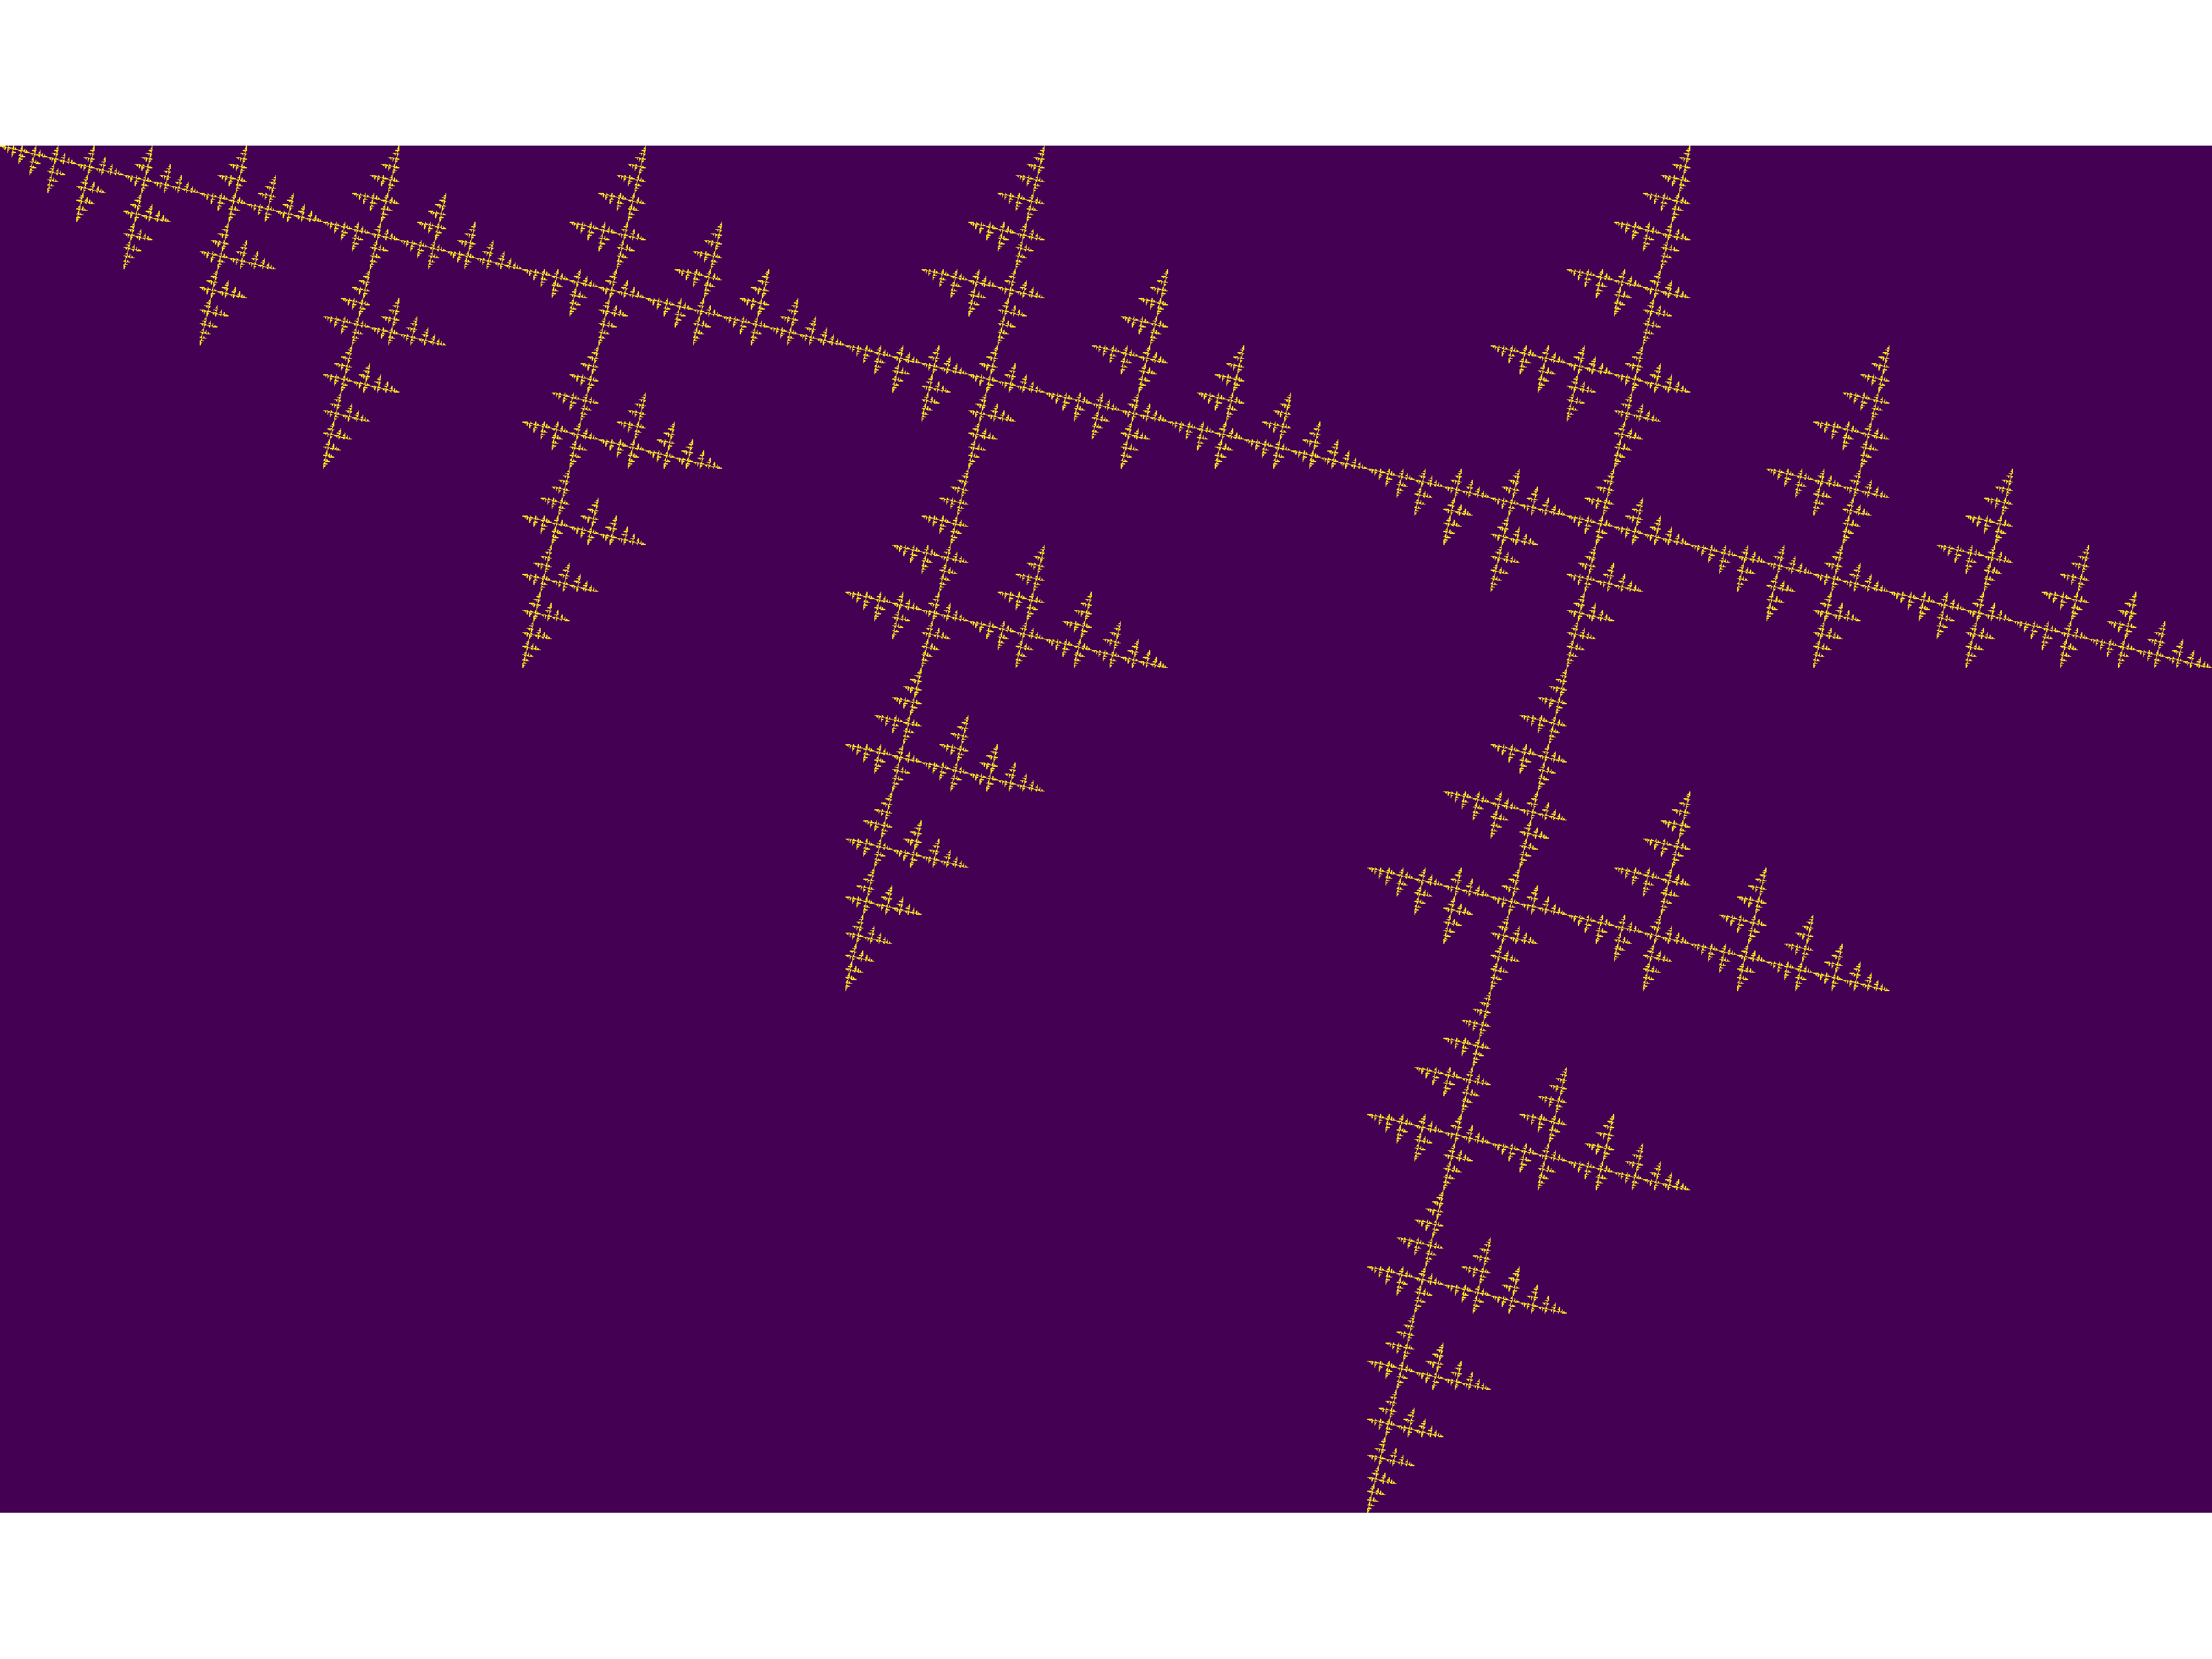
\includegraphics[width=9cm]{../Problems/fractal-dimensions/my-self-rep-frac-GR.png}
\caption{\label{My-Frac-GR}Fractal that emerges by Rotating and appending boxes, this demonstrates the relationship between the Fibonacci numbers and golden ratio very well}
\end{figure}

\begin{figure}[htbp]
\centering
\includesvg[width=9cm]{../Problems/fractal-dimensions/My-Fib-Fractal-Diagram}
\caption{\label{My-Frac-GR}Fractal that emerges by Rotating and appending boxes, this demonstrates the relationship between the Fibonacci numbers and golden ratio very well}
\end{figure}

\subsection{Discuss Pattern shows Fibonacci Numbers}
\label{sec:orgbe11c04}
\subsubsection{Angle Relates to Golden Ratio}
\label{sec:org1b634b9}
\subsection{Prove Fibonacci using Monotone Convergence Theorem}
\label{sec:org645dc7b}
Consider the series:

$$\begin{aligned}
G_n &= \frac{F_{n} }{F_{n - 1} } \\
\end{aligned}$$

Such that:

$$\begin{aligned}
F_n = F_{n- 1} +  F_{n- 2} ; \quad F_1 = F_2 = 1
\end{aligned}$$


\subsubsection{Show that the Series is Monotone}
\label{sec:org2528a11}
$$\begin{aligned}
F_{n} &> 0 \\
0 &< F_{n} \\
 \implies   0 &< F_{n - 2} +  F_{n- 1} \quad \forall n > 2 \\
  F_{n- 2} &< F_{n- 1}  \\
   \implies  F_n & < F_{n+1}
\end{aligned}$$

$$\begin{aligned}
F_{n} &> 0 \\
0 &< F_{n} \\
 \implies   0 &< F_{n - 2} +  F_{n- 1} \quad \forall n > 2 \\
  F_{n- 2} &< F_{n- 1}  \\
   \implies  F_n & < F_{n+1}
\end{aligned}$$



\subsubsection{Show that the Series is Bounded}
\label{sec:orgc8f7e2c}
\subsubsection{Find the Limit}
\label{sec:org2640962}
$$\begin{aligned}
G &= \frac{F_{n} +  F_{n+  1} }{F_{n+  1} } \\
&= 1 +  \frac{F_{n- 1} }{F_n} \\
\text{Recall that $F_n > 0 \forall n$}\\
&=  1 +  \frac{1}{    \left\lvert G \right\rvert } \\
 \implies  0 &= G^2- G +  1; \quad G > 0  \\
  \implies  G = \varphi &=  \frac{\sqrt{5} - 1  }{2} \quad  \square
\end{aligned}$$


\subsubsection{Comments}
\label{sec:orgc6a1d24}

The Fibonacci sequence is quite unique, observe that:

This can be rearranged to show that the Fibonacci sequence is itself
when shifted in either direction, it is the sequence that does not
change during recursion.

\[\begin{aligned}
F_{n+ 1} - F_{n} = F_{n- 1} \quad \forall n > 1
\end{aligned}\]

This is analogous to how \(e^x\) doesn't change under differentiation:

$$\begin{aligned}
\frac{\mathrm{d} }{\mathrm{d} x}\left( e^x \right) \ldots
\end{aligned}$$

or how 0 is the additive identity and it shows why generating functions
are so useful.

Observe also that

$$\begin{aligned}
\lim_{n     \rightarrow \infty }\left[ \frac{F_n}{F_{n- 1} }  \right] &= \varphi \\
\lim_{n     \rightarrow \infty }\left[ \frac{F_n}{F_{n- 1} }  \right] &= \psi \\
\varphi - \psi &=  1 \\
\varphi \times  \psi  &= 1 \\
\frac{\psi}{\varphi}  = \frac{1}{\varphi^2} = \frac{1}{1-\varphi} &= \frac{1}{2-\varphi} = \frac{2}{3 - \sqrt{5}  }
\end{aligned}$$
\subsubsection{Python}
\label{sec:orge4a6275}

\begin{minted}[]{python}
#+begin_src python
import matplotlib.pyplot as plt
import sympy

plt.plot([ sympy.N(sympy.fibonacci(n+1)/sympy.fibonacci(n)) for n in range(1, 30)])
plt.savefig("./a.png")
\end{minted}
\begin{center}
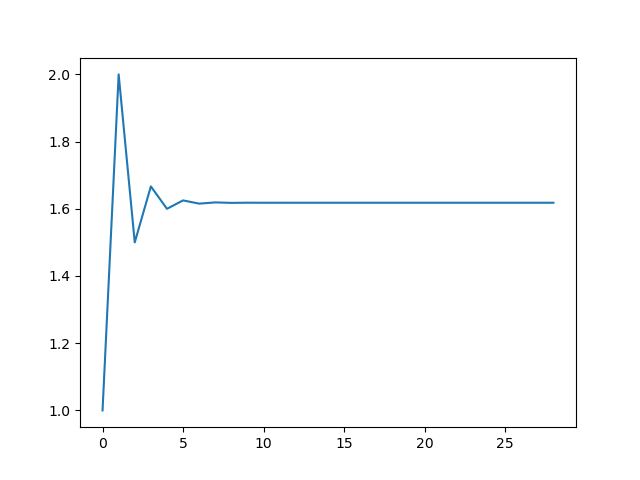
\includegraphics[width=.9\linewidth]{./a.png}
\end{center}

\subsection{Angle is \(\tan^{-1}\left( \frac{1}{1-\varphi}\right)\)}
\label{sec:orgfd164c2}
\subsubsection{Similar to Golden Angle \(2 \pi \left( \frac{1}{1-\varphi}\right)\)}
\label{sec:org345967f}
\subsection{Dimension of my Fractal}
\label{sec:orgeb352d2}
\(\log_{\varphi}(2)\)
\subsection{Code should be split up or put into appendix}
\label{sec:org0812b9b}
\begin{minted}[]{julia}
function matJoin(A, B)
    function nrow(X)
        return size(X)[1]
    end
    function ncol(X)
        return size(X)[2]
    end
    emptymat = zeros(Bool, max(size(A)[1], size(B)[1]) ,sum(ncol(A) + ncol(B)) )
    emptymat[1:nrow(A), 1:ncol(A)] = A
    emptymat[1:nrow(B), (ncol(A)+1):ncol(emptymat)] = B
    return emptymat
end

function mywalk(B, n)
    for i in 1:n
        B = matJoin(B, rotl90(B));
    end
    return B
end

############################################################
##### Use Plot for themes ##################################
############################################################

using Plots
# SavePlot
## Docstring
    """
# MakePlot
Saveplot will save a plot of the fractals

- `n`
  - Is the number of iterations to produce the fractal
    - ``\\frac{n!}{k!(n - k)!} = \\binom{n}{k}``
- `filename`
  - Is the File name
- `backend`
  - either `gr()` or `pyplot()`
    - Gr is faster
    - pyplot has lines
    - Avoiding this entirely and using `GR.image()` and
     `GR.savefig` is even faster but there is no support
     for changing the colour schemes

    """
function makePlot(n, backend=pyplot())
    backend
    plt = Plots.plot(mywalk([1 1], n),
                     st=:heatmap, clim=(0,1),
                     color=:coolwarm,
                    colorbar_title="", ticks = true, legend = false, yflip = true, fmt = :svg)
    return plt
end
plt = makePlot(5)

"""
# savePlot
Saves a Plot created with `Plots.jl` to disk (regardless of backend) as both an
svg, use ImageMagick to get a PNG if necessary

- `filename`
  - Location on disk to save image
- `plt`
  - A Plot object created by using `Plot.jl`
"""
function savePlot(filename, plt)
    filename = replace(filename, " " => "_")
    path = string(filename, ".svg")
    Plots.savefig(plt, path)
    print("Image saved to ", path)
end

#------------------------------------------------------------
#-- Dimension -----------------------------------------------
#------------------------------------------------------------
# Each time it iterates the image scales by phi
# and the number of pixels increases by 2
# so log(2)/log(1.618)
# lim(F_n/F_n-1)
# but the overall dimensions of the square increases by a factor of 3
# so 3^D=5 ==> log_3(5) = log(5)/log(3) = D
using DataFrames
function returnDim()
    mat2 = mywalk(fill(1, 1, 1), 10)
    l2   = sum(mat2)
    size2 = size(mat2)[1]
    mat1 = mywalk(fill(1, 1, 1), 11)
    l1   = sum(mat1)
    size1 = size(mat1)[1]
    df = DataFrame
    df.measure = [log(l2/l1)/log(size2/size1)]
    df.actual  = [log(2)/log(1.618) ]
    return df
end

############################################################
### Main Functions ##########################################
############################################################
# Usually Main should go into a seperate .jl filename
# Then a compination of import, using, include will
# get the desired effect of top down programming.
# Combine this with using a tmp.jl and tst.jl and you're set.
# See https://stackoverflow.com/a/24935352/12843551
# http://ryansnotes.org/mediawiki/index.php/Workflow_Tips_in_Julia

# Produce and Save a Plot
#=
filename = "my-self-rep-frac";
filename = string(pwd(), "/", filename);
savePlot(filename, makePlot(5))
;convert $filename.svg $filename.png
makePlot(5, pyplot())
=#
# Return the Dimensions
returnDim()


############################################################
#### Render Image ##########################################
#################yellow and purple##########################
using GR
GR.imshow(mywalk([1 1], 5))


\end{minted}

\section{The Fibonacci Sequence}
\label{sec:org52ccdb8}
The Fibonacci Sequence occurs in my example from the \S \ref{my-fractal}, let's investigate it
\subsection{Introduction}
\label{sec:orga22c5d5}
The \emph{Fibonacci Sequence} and \emph{Golden Ratio} share a deep connection\footnote{See section} and occur in patterns observed in nature very frequently
(see
\cite{shellyallenFibonacciNature,benedettapalazzoNumbersNatureFibonacci2016,MinarovaNikoletta2014TFSN,NatureGoldenRatio2018,robertlambHowAreFibonacci2008,ronknottFibonacciNumbersGolden2016}), an example of such an occurence is discussed in section \ref{sunflower-example}.


In this section we lay out a strategy to find an analytic solution to the
\emph{Fibonacci Sequence} by relating it to a continuous series and generalise this
approach to any homogenous linear recurrence relation.

This details some open mathematical work for the project and our hope is that by
identifying relationships between discrete and continuous systems generall we
will be able to draw insights with regard to the occurrence of patterns related
to the \emph{Fibonacci Sequence} and \emph{Golden Ratio} in nature.

\subsection{Computational Approach}
\label{define-the-fibonacci-numbers}
Given that much of our work will involve computational analysis and simulation we begin with a strategy to solve the sequence computationally.

The \emph{Fibonacci} Numbers are given by:

\begin{align}
F_n = F_{n-1} + F_{n-2} \label{eq:fib-def}
\end{align}

This type of recursive relation can be expressed in \emph{Python} by using recursion,
as shown in listing \ref{fib-rec-0}, however using this function will reveal that it
is extraordinarily slow, as shown in listing \ref{time-slow}, this is because the
results of the function are not cached and every time the function is called
every value is recalculated\footnote{Dr. Hazrat mentions something similar in his book with respect to
\emph{Mathematica}\textsuperscript{\textregistered}
\cite[Ch. 13]{hazratMathematicaProblemCenteredApproach2015}}, meaning that the workload scales in
exponential as opposed to polynomial time.

The \texttt{functools} library for python includes the \texttt{@functools.lru\_cache} decorator
which will modify a defined function to cache results in memory
\cite{FunctoolsHigherorderFunctions}, this means that the recursive function will
only need to calculate each result once and it will hence scale in polynomial
time, this is implemented in listing \ref{fib-cache}.


\begin{listing}[htbp]
\begin{minted}[]{python}
  def rec_fib(k):
      if type(k) is not int:
          print("Error: Require integer values")
          return 0
      elif k == 0:
          return 0
      elif k <= 2:
          return 1
      return rec_fib(k-1) + rec_fib(k-2)
\end{minted}
\caption{\label{fib-rec-0}Defining the \emph{Fibonacci Sequence} \eqref{eq:fib-def} using Recursion}
\end{listing}

\begin{listing}[htbp]
\begin{minted}[]{python}
  start = time.time()
  rec_fib(35)
  print(str(round(time.time() - start, 3)) + "seconds")

## 2.245seconds
\end{minted}
\caption{\label{time-slow}Using the function from listing \ref{fib-rec-0} is quite slow.}
\end{listing}


\begin{listing}[htbp]
\begin{minted}[]{python}
  from functools import lru_cache

  @lru_cache(maxsize=9999)
  def rec_fib(k):
      if type(k) is not int:
          print("Error: Require Integer Values")
          return 0
      elif k == 0:
          return 0
      elif k <= 2:
          return 1
      return rec_fib(k-1) + rec_fib(k-2)


start = time.time()
rec_fib(35)
print(str(round(time.time() - start, 3)) + "seconds")
## 0.0seconds
\end{minted}
\caption{\label{fib-cache}Caching the results of the function previously defined \ref{time-slow}}
\end{listing}

\begin{minted}[]{python}
  start = time.time()
  rec_fib(6000)
  print(str(round(time.time() - start, 9)) + "seconds")

## 8.3923e-05seconds
\end{minted}

Restructuring the problem to use iteration will allow for even greater performance as demonstrated by finding \(F_{10^{6}}\) in listing \ref{fib-iter}. Using a compiled language such as \emph{Julia} however would be thousands of times faster still, as demonstrated in listing \ref{julia-fib}.



\begin{listing}[htbp]
\begin{minted}[]{python}
  def my_it_fib(k):
      if k == 0:
          return k
      elif type(k) is not int:
          print("ERROR: Integer Required")
          return 0
      # Hence k must be a positive integer

      i  = 1
      n1 = 1
      n2 = 1

      # if k <=2:
      #     return 1

      while i < k:
         no = n1
         n1 = n2
         n2 = no + n2
         i = i + 1
      return (n1)

  start = time.time()
  my_it_fib(10**6)
  print(str(round(time.time() - start, 9)) + "seconds")

 ## 6.975890398seconds
\end{minted}
\caption{\label{fib-iter}Using Iteration to Solve the Fibonacci Sequence}
\end{listing}

\begin{listing}[htbp]
\begin{minted}[]{julia}
function my_it_fib(k)
    if k == 0
        return k
    elseif typeof(k) != Int
        print("ERROR: Integer Required")
        return 0
    end
    # Hence k must be a positive integer

    i  = 1
    n1 = 1
    n2 = 1

    # if k <=2:
    #     return 1
    while i < k
       no = n1
       n1 = n2
       n2 = no + n2
       i = i + 1
    end
    return (n1)
end

@time my_it_fib(10^6)

##  my_it_fib (generic function with 1 method)
##    0.000450 seconds
\end{minted}
\caption{\label{julia-fib}Using Julia with an iterative approach to solve the 1 millionth fibonacci number}
\end{listing}

In this case however an analytic solution can be found by relating discrete
mathematical problems to continuous ones as discussed below at section .
\subsection{Exponential Generating Functions}
\label{exp-gen-func-fib-seq}
\paragraph{Motivation}
\label{motivation}
Consider the \emph{Fibonacci Sequence} from \eqref{eq:fib-def}:


\begin\{aLign
    a\textsubscript{n}\&= a\textsubscript{n - 1} + a\textsubscript{n - 2} \nonumber \\
\iff a\textsubscript{n+  2} \&= a\textsubscript{n+  1} +  a\textsubscript{n} \label{eq:fib-def-shift}
\end{align}


from observation, this appears similar in structure to the following \emph{ordinary
differential equation}, which would be fairly easy to deal with:


\begin{align*}
f''\left( x \right)- f'\left( x \right)- f\left( x \right)=  0
\end{align*}

By ODE Theory we have \(y \propto e^{m_{i}x}, \enspace i = 1, 2\):

\begin{align*}
f\left( x \right)= e^{mx} = \sum^{\infty}_{n= 0}   \left[ r^{m} \frac{x^n}{n!} \right]
\end{align*}

So using some sort of a transformation involving a power series may help to
relate the discrete problem back to a continuous one.

\paragraph{Example}
\label{solving-the-sequence}
Consider using the following generating function, (proof of the
generating function derivative as in \eqref{eq:exp-gen-def-2} and \eqref{eq:exp-gen-def-3} is
provided in section \ref{Derivative-exp-gen-function})




\begin{align}
    f\left( x \right) &=  \sum^{\infty}_{n= 0}   \left[ a_{n} \cdot  \frac{x^n}{n!} \right]   \label{eq:exp-gen-def-1} \\
 \implies   f'\left( x \right) &=  \sum^{\infty}_{n= 0}   \left[ a_{n+1} \cdot  \frac{x^n}{n!} \right]   \label{eq:exp-gen-def-2} \\
\implies    f''\left( x \right) &=  \sum^{\infty}_{n= 0}   \left[ a_{n+2} \cdot  \frac{x^n}{n!} \right]   \label{eq:exp-gen-def-3}
\end{align}


So the Fibonacci recursive relation from \eqref{eq:fib-def-shift}  could be expressed :


\begin{align*}
a_{n+  2}    &= a_{n+  1} +  a_{n}\\
\frac{x^n}{n!}   a_{n+  2}    &= \frac{x^n}{n!}\left( a_{n+  1} +  a_{n}  \right)\\
\sum^{\infty}_{n= 0} \left[ \frac{x^n}{n!}   a_{n+  2} \right]        &= \sum^{\infty}_{n= 0}   \left[ \frac{x^n}{n!} a_{n+  1} \right]  + \sum^{\infty}_{n= 0}   \left[ \frac{x^n}{n!} a_{n}  \right]  \\
\end{align*}

And hence by applying \eqref{eq:exp-gen-def-1}, \eqref{eq:exp-gen-def-2} and \eqref{eq:exp-gen-def-3}:

\begin{align}
f''\left( x \right) &= f'\left( x \right)+  f\left( x \right)
\end{align}


Using the theory of higher order linear differential equations with
constant coefficients it can be shown:


\begin{align*}
f\left( x \right)= c_1 \cdot  \mathrm{exp}\left[ \left( \frac{1- \sqrt{5} }{2} \right)x \right] +  c_2 \cdot  \mathrm{exp}\left[ \left( \frac{1 +  \sqrt{5} }{2} \right)x \right]
\end{align*}


By equating this to the power series:


\begin{align*}
f\left( x \right)&= \sum^{\infty}_{n= 0}   \left[ \left( c_1\left( \frac{1- \sqrt{5} }{2} \right)^n +  c_2  \left( \frac{1+ \sqrt{5} }{2} \right)^n \right) \cdot  \frac{x^n}{n!} \right]
\end{align*}


Now given that:


\begin{align*}
f\left( x \right)= \sum^{\infty}_{n= 0}   \left[ a_n \frac{x^n}{n!} \right]
\end{align*}


We can conclude that:


\begin{align*}
a_n = c_1\cdot  \left( \frac{1- \sqrt{5} }{2} \right)^n +  c_2 \cdot  \left( \frac{1+  \sqrt{5} }{2} \right)^n
\end{align*}


By applying the initial conditions:


\begin{align*}
a_0= c_1 +  c_2  \implies  c_1= - c_2\\
a_1= c_1 \left( \frac{1+ \sqrt{5} }{2} \right) -  c_1 \left( \frac{1-\sqrt{5} }{2} \right)  \implies  c_1 = \frac{1}{\sqrt{5} }\\
\therefore ~ c_1 = \frac{1}{\sqrt{5}, ~ c_2 = -\frac{1}{\sqrt{5}}}
\end{align*}


And so finally we have the solution to the \emph{Fibonacci Sequence} \ref{eq:fib-def-shift}:


\begin{align}
    a_n &= \frac{1}{\sqrt{5} } \left[ \left( \frac{1+  \sqrt{5} }{2}  \right)^n -  \left( \frac{1- \sqrt{5} }{2} \right)^n \right] \nonumber \\
&= \frac{\varphi^n - \psi^n}{\sqrt{5} } \nonumber\\
&=\frac{\varphi^n -  \psi^n}{\varphi - \psi} \label{eq:fib-sol}
\end{align}


where:

\begin{itemize}
\item \(\varphi = \frac{1+ \sqrt{5} }{2} \approx 1.61\ldots\)
\item \(\psi = 1-\varphi = \frac{1- \sqrt{5} }{2} \approx 0.61\ldots\)
\end{itemize}

\paragraph{Derivative of the Exponential Generating Function}
\label{Derivative-exp-gen-function}
\subparagraph{Base}
\label{sec:orgb7d7577}
Differentiating the exponential generating function has the effect of shifting the sequence once to the left: \cite{lehmanReadingsMathematicsComputer2010}

\begin{align}
    f\left( x \right) &= \sum^{\infty}_{n= 0}   \left[ a_n \frac{x^n}{n!} \right] \label{eq:exp-pow-series} \\
f'\left( x \right) &= \frac{\mathrm{d} }{\mathrm{d} x}\left( \sum^{\infty}_{n= 0}   \left[ a_n \frac{x^n}{n!} \right]  \right) \nonumber \\
&= \frac{\mathrm{d}}{\mathrm{d} x} \left( a_0 \frac{x^0}{0!} +  a_1 \frac{x^1}{1!} +  a_2 \frac{x^2}{2!}+  a_3 \frac{x^3}{3! } +  \ldots \frac{x^k}{k!} \right) \nonumber \\
&= \sum^{\infty}_{n= 0}   \left[ \frac{\mathrm{d} }{\mathrm{d} x}\left( a_n \frac{x^n}{n!} \right) \right] \nonumber \\
&= \sum^{\infty}_{n= 0}   {\left[{ \frac{a_n}{{\left({ n- 1 }\right)!}} } x^{n- 1}  \right]} \nonumber \\
\implies f'(x) &= \sum^{\infty}_{n= 1}   {\left[{ \frac{x^n}{n!}a_{n+  1} }\right]} \label{eq:exp-pow-series-sol}
\end{align}

\subparagraph{Bridge}
\label{sec:orga903342}
This can be shown for all derivatives by way of induction, for

\begin{align}
f^{(k)}\left(x\right) = \sum_{n=k}^\infty\frac{a_{n+k}\cdot x^n}{n!} \quad \text{for}~k \ge 0
\end{align}

Assume that \(f^{(k)}\left(x\right) = \sum_{n=k}^\infty\frac{a_{n+k}\cdot x^n}{n!}\)

Using this assumption, prove for the next element \(k+1\)

We need \(f^{(k+1)}(x) = \sum_{n=k+1}^\infty\frac{a_{n+k+1}\cdot x^n}{n!}\)

\begin{align*}
    \text{LHS} &= f^{(k+1)}(x)\\
    &= \frac{\mathrm{d}}{\mathrm{d}x}\left(f^{(k)}(x)\right)\\
    &= \frac{\mathrm{d}}{\mathrm{d}x}\left(\sum_{n=k}^\infty\frac{a_{n+k}\cdot x^n}{n!}\right)\quad \text{by assumption}\\
    &= \sum_{n=k}^\infty\frac{a_{n+k}\cdot n\cdot x^{n-1}}{n!}\\
    &= \sum_{n=k}^\infty\frac{a_{n+k}\cdot x^{n-1}}{(n-1)!}\\
    &= \sum_{n=k+1}^\infty\frac{a_{n+k+1}\cdot x^{n}}{n!}\\
    &= \text{RHS}
\end{align*}

Therefore, by mathematical induction \(f^{(k)}\left(x\right) = \sum_{n=k}^\infty\frac{a_{n+k}\cdot x^n}{n!} \quad \text{for}~k \ge 0\)

Furthermore, if the first derivative of the exponential generating function shown in \eqref{eq:exp-pow-series-sol}
shifts the sequence across, then every derivative thereafter does so as well.

\paragraph{Homogeneous Proof}
\label{sec:org71f107b}
An equation of the form:

\begin{align}
\sum^{n}_{i=0} \left[ c_{i} \cdot f^{(i)}(x) \right] = 0 \label{eq:hom-ode}
\end{align}

is said to be a homogenous linear ODE: \cite[Ch. 2]{zillDifferentialEquations2009a}

\begin{description}
\item[{Linear}] because the equation is linear with respect to \(f(x)\)
\item[{Ordinary}] because there are no partial derivatives (e.g. \(\frac{\partial }{\partial x}{\left({ f{\left({ x }\right)} }\right)}\)  )
\item[{Differential}] because the derivates of the function are concerned
\item[{Homogenous}] because the \textbf{\emph{RHS}} is 0
\begin{itemize}
\item A non-homogeous equation would have a non-zero RHS
\end{itemize}
\end{description}

There will be \(k\) solutions to a \(k^{\mathrm{th}}\) order linear ODE, each may be summed to produce a superposition which will also be a solution to the equation, \cite[Ch. 4]{zillDifferentialEquations2009a}  this will be considered as the desired complete solution (and this will be shown to be the only solution for the recurrence relation \eqref{eq:recurrence-relation-def}. These \(k\) solutions will be in one of two forms:

\begin{enumerate}
\item \(f(x)=c_{i} \cdot e^{m_{i}x}\)
\item \(f(x)=c_{i} \cdot x^{j}\cdot e^{m_{i}x}\)
\end{enumerate}

where:

\begin{itemize}
\item \(\sum^{k}_{i=0}\left[  c_{i}m^{k-i} \right] = 0\)
\begin{itemize}
\item This is referred to the characteristic equation of the recurrence relation or ODE \cite{levinSolvingRecurrenceRelations2018}
\end{itemize}
\item \(\exists i,j \in \mathbb{Z}^{+} \cap \left[0,k\right]\)
\begin{itemize}
\item These are often referred to as repeated roots \cite{levinSolvingRecurrenceRelations2018,zillMatrixExponential2009} with a multiplicity corresponding to the number of repetitions of that root \cite[\textsection 3.2]{nicodemiIntroductionAbstractAlgebra2007}
\end{itemize}
\end{itemize}

\subparagraph{Unique Roots of Characteristic Equation}
\label{uniq-roots-recurrence}
\begin{enumerate}
\item Example
\label{sec:orgf440bd1}
An example of a recurrence relation with all unique roots is the fibonacci sequence, as described in section \ref{solving-the-sequence}.
\item Proof
\label{sec:org33cbec6}
Consider the linear recurrence relation \eqref{eq:recurrence-relation-def}:

\begin{align}
\sum^{n}_{i= 0}   \left[ c_i \cdot  a_i \right] = 0, \quad \exists c \in
\mathbb{R}, \enspace \forall i<k\in\mathbb{Z}^+ \nonumber \label{eq:recurrence-relation-def}
\end{align}
This implies:


\begin{align}
    \sum^{\infty}_{n= 0}   \left[ \sum^{k}_{i= 0}   \left[ \frac{x^n}{n!} c_i a_n \right]  \right]  &= 0 \\
    \sum^{\infty}_{n= 0}    \sum^{k}_{i= 0}    \frac{x^n}{n!} c_i a_n    &= 0 \\
        \sum^{k}_{i= 0} c_i \sum^{\infty}_{n= 0}    \frac{x^n}{n!}  a_n    &= 0
\end{align}

By implementing the exponential generating function as shown in
\eqref{eq:exp-gen-def-1}, this provides:

\begin{align}
   \sum^{k}_{i= 0}   \left[ c_i f^{\left( i \right)}\left( x \right) \right]
\end{align}


Now assume that the solution exists and all roots of the characteristic polynomial are unique (i.e. the solution is of the form \(f{\left({ x }\right)} \propto e^{m_i x}: \quad m_i \neq m_j \forall i\neq j\)), this implies that  \cite[Ch. 4]{zillDifferentialEquations2009a} :

\begin{align}
    f{\left({ x }\right)} = \sum^{k}_{i= 0}   {\left[{ k_i e^{m_i x} }\right]}, \quad \exists m,k \in \mathbb{C} \nonumber
\end{align}

This can be re-expressed in terms of the exponential power series, in order to relate the solution of the function \(f{\left({ x }\right)}\) back to a solution of the sequence \(a_n\), (see section for a derivation of the exponential power series \textbf{\#TODO make section on to prove exponential power series using taylor series expansion if we get time)}:

\begin{align}
    \sum^{k}_{i= 0}   {\left[{ k_i e^{m_i x}  }\right]}  &= \sum^{k}_{i= 0}   {\left[{ k_i \sum^{\infty}_{n= 0}   \frac{{\left({ m_i x }\right)}^n}{n!}  }\right]}  \nonumber \\
							 &= \sum^{k}_{i= 0}  \sum^{\infty}_{n= 0}   k_i m_i^n \frac{x^n}{n!} \nonumber\\
							 &=    \sum^{\infty}_{n= 0} \sum^{k}_{i= 0}   k_i m_i^n \frac{x^n}{n!} \nonumber \\
							 &= \sum^{\infty}_{n= 0} {\left[{ \frac{x^n}{n!}  \sum^{k}_{i=0}   {\left[{ k_im^n_i }\right]}  }\right]}, \quad \exists k_i \in \mathbb{C}, \enspace \forall i \in \mathbb{Z}^+\cap {\left[{ 1, k }\right]}     \label{eq:unique-root-sol-power-series-form}
\end{align}


Recall the definition of the generating function from \eqref{eq:exp-gen-def-1}, by equating this to \eqref{eq:unique-root-sol-power-series-form}:

\begin{align}
    f{\left({ x }\right)} &= \sum^{\infty}_{n= 0}   {\left[{  \frac{x^n}{n!} a_n }\right]} \nonumber \\
&= \sum^{\infty}_{n= 0} {\left[{ \frac{x^n}{n!}  \sum^{k}_{i=0}   {\left[{ k_im^n_i }\right]}  }\right]}  \nonumber \\
      \implies  a_n &= \sum^{k}_{n= 0} {\left[{ k_im_i^n }\right]}     \nonumber \\ \nonumber
\square
\end{align}

This can be verified by the fibonacci sequence as shown in section \ref{solving-the-sequence}, the solution to the characteristic equation is \(m_1 = \varphi, m_2 = {\left({ 1-\varphi }\right)}\) and the corresponding solution to the linear ODE and recursive relation are:

\begin{alignat}{4}
    f{\left({ x }\right)} &= &c_1 e^{\varphi x} +  &c_2 e^{{\left({ 1-\varphi }\right)} x}, \quad &\exists c_1, c_2 \in \mathbb{R} \subset \mathbb{C} \nonumber \\
    \iff  a_n &= &k_1 n^{\varphi} +  &k_2 n^{1- \varphi}, &\exists k_1, k_2 \in \mathbb{R} \subset \mathbb{C} \nonumber
\end{alignat}
\end{enumerate}

\subparagraph{Repeated Roots of Characteristic Equation}
\label{rep-roots-recurrence}
\begin{enumerate}
\item Example
\label{sec:org370dd94}
Consider the following recurrence relation:

\begin{align}
    a_{n+2} -  10a_{n+ 1} +  25a_{n}&= 0 \label{eq:hom-repeated-roots-recurrence} \\
    \implies  \sum^{\infty}_{n= 0}   {\left[{ a_{n+2} \frac{x^n}{n!} }\right]} - 10 \sum^{\infty}_{n= 0}   {\left[{ a_{n+1} \frac{x^n}{n!}    }\right]} + 25 \sum^{\infty}_{n= 0 }   {\left[{  a_{n}\frac{x^n}{n!} }\right]}&= 0 \nonumber
\end{align}

By applying the definition of the exponential generating function at \eqref{eq:exp-gen-def-1} :

\begin{align}
    f''{\left({ x }\right)}- 10f'{\left({ x }\right)}+  25f{\left({ x }\right)}= 0 \label{eq:rep-roots-func-ode}
\end{align}

By implementing the already well-established theory of linear ODE's, the
characteristic equation for \eqref{eq:rep-roots-func-ode} can be expressed as:

\begin{align}
    m^2- 10m+  25 = 0 \nonumber \\
    {\left({ m- 5 }\right)}^2 = 0 \nonumber \\
    m= 5 \label{eq:rep-roots-recurrence-char-sol}
\end{align}

Herein lies a complexity, in order to solve this, the solution produced from \eqref{eq:rep-roots-recurrence-char-sol} can be used with the \emph{Reduction of Order} technique to produce a solution that will be of the form \cite[\textsection 4.3]{zillMatrixExponential2009}.

\begin{align}
    f{\left({ x }\right)}= c_1e^{5x} +  c_2 x e^{5x} \label{eq:rep-roots-ode-sol}
\end{align}

\eqref{eq:rep-roots-ode-sol} can be expressed in terms of the exponential power series in order to try and relate the solution for the function back to the generating function,
observe however the following power series identity (proof in section \ref{prove-general-exp-identity}):

\begin{align}
    x^ke^x &= \sum^{\infty}_{n= k}   {\left[{ \frac{x^n}{{\left({ n- k }\right)}!} }\right]}, \quad \exists k \in \mathbb{Z}^+ \label{eq:uniq-roots-pow-series-ident}
\end{align}

by applying identity \eqref{eq:uniq-roots-pow-series-ident} to equation \eqref{eq:rep-roots-ode-sol}

\begin{align}
    \implies  f{\left({ x }\right)} &= \sum^{\infty}_{n= 0}   {\left[{ c_1 \frac{{\left({ 5x }\right)}^n}{n!} }\right]}  +  \sum^{\infty}_{n= 1}   {\left[{ c_2 n \frac{{\left({ 5x }\right)^n}}{n{\left({ n-1 }\right)}!} }\right]} \nonumber \\
 &= \sum^{\infty}_{n= 0}   {\left[{ \frac{x^n}{n!} {\left({ c_{1}5^n +  c_2 n 5^n   }\right)} }\right]} \nonumber
\end{align}

Given the defenition of the exponential generating function from \eqref{eq:exp-gen-def-1}

\begin{align}
    f{\left({ x }\right)}&=     \sum^{\infty}_{n= 0}   {\left[{ a_n \frac{x^n}{n!} }\right]} \nonumber \\
    \iff a_n &= c_{1}5^n +  c_{2}5^n \nonumber \\ \nonumber
    \ \nonumber \\
    \square \nonumber
\end{align}

\item Proof
\label{sec:orga27a822}
Consider a recurrence relation of the form:

\begin{align}
     \sum^{k}_{n= 0}   {\left[{ c_i a_n }\right]}  = 0 \nonumber \\
      \implies  \sum^{\infty}_{n= 0}   \sum^{k}_{i= 0}   c_i a_n \frac{x^n}{n!} = 0 \nonumber \\
      \sum^{k}_{i= 0}   \sum^{\infty}_{n= 0}   c_i a_n \frac{x^n}{n!} \nonumber
\end{align}

By substituting for the value of the generating function from \eqref{eq:exp-gen-def-1}:

\begin{align}
    \sum^{k}_{i= 0}   {\left[{ c_if^{{\left({ k }\right)}}  {\left({ x }\right)}    }\right]} \label{eq:gen-form-rep-roots-ode}
\end{align}

Assume that \eqref{eq:gen-form-rep-roots-ode} corresponds to a charecteristic polynomial with only 1 root of multiplicity \(k\), the solution would hence be of the form:

\begin{align}
			 & \sum^{k}_{i= 0}   {\left[{ c_i m^i }\right]} = 0 \wedge m=B, \enspace  \exists! B \in \mathbb{C} \nonumber \\
 \implies      f{\left({ x }\right)}&= \sum^{k}_{i= 0}   {\left[{ x^i A_i e^{mx} }\right]}, \quad \exists A \in \mathbb{C}^+, \enspace \forall i \in {\left[{ 1,k }\right]} \cap \mathbb{N}  \label{eq:sol-rep-roots-ode}
\end{align}

If we assume the identity from \eqref{eq:uniq-roots-pow-series-ident}:

\begin{align}
x^k e^x = \sum^{\infty}_{n= k} {\left[{ \frac{x^n}{{\left({ n- k }\right)}!} }\right]}  \nonumber
\end{align}

See section \ref{prove-general-exp-identity} for proof.

We can apply identity \eqref{eq:uniq-roots-pow-series-ident} to \eqref{eq:sol-rep-roots-ode}, which gives:

\begin{align}
f{\left({ x }\right)}&=     \sum^{k}_{i= 0}   {\left[{ A_i \sum^{\infty}_{n= i}   {\left[{ \frac{{\left({ x m }\right)}^n}{{\left({ n- i }\right)}!} }\right]}  }\right]} \nonumber \\
&=     \sum^{\infty}_{n= 0}   {\left[{ \sum^{k}_{i=0} {\left[{ \frac{x^n}{n!}  \frac{n!}{{\left({ n- i }\right)!}} A_i m^n }\right]}       }\right]} \nonumber \\
&=     \sum^{\infty}_{n= 0} {\left[{ \frac{x^n}{n!}   \sum^{k}_{i=0} {\left[{  \frac{n!}{{\left({ n- i }\right)!}} A_i m^n }\right]}       }\right]} \nonumber
\end{align}

Recall the generating function that was used to get \eqref{eq:gen-form-rep-roots-ode}:

\begin{align}
f{\left({ x }\right)}&= \sum^{\infty}_{n= 0}   {\left[{ a_n \frac{x^n}{n!} }\right]}      \nonumber \\
 \implies  a_n &= \sum^{k}_{i= 0}   {\left[{ A_i \frac{n!}{{\left({ n- i }\right)}!} m^n  }\right]} \nonumber \\
 &= \sum^{k}_{i= 0}   {\left[{ m^n A_i \prod_{0}^{k} {\left[{ n- {\left({ i- 1 }\right)} }\right]}   }\right]}
& \intertext{$\because \enspace i \leq k$} \notag \nonumber \\
 &= \sum^{k}_{i= 0} {\left[{ A_i^* m^n n^i }\right]}, \quad \exists A_i \in \mathbb{C}, \enspace \forall i\leqk \in \mathbb{Z}^+ \nonumber \\
\ \nonumber \\
\square \nonumber
\end{align}

\item Proof
\label{prove-general-exp-identity}
In this section the proof of
\begin{enumerate}
\item Motivation
\label{sec:orgc24b4f7}

Consider the function \(f(x) = xe^x\). Using the taylor series formula we get the following:

\begin{align*}
    xe^x &= 0+\frac{1}{1!}x+\frac{2}{2!}x^2+\frac{3}{3!}x^3+\frac{4}{4!}x^4+\frac{5}{5!}x^5+\dots\\
    &= \sum_{n=0}^\infty \frac{nx^n}{n!}\\
    &= \sum_{n=1}^\infty \frac{x^n}{(n-1)!}
\end{align*}

Similarly, \(f(x) = x^2e^x\) will give:
\begin{align*}
    x^2e^x &= \frac{0}{0!} + \frac{0x}{1!} + \frac{2x^2}{2!} + \frac{6x^3}{3!} + \frac{12x^4}{4!} + \frac{20x^5}{5!} + \dots\\
    &= \frac{2\cdot 1x^2}{2!} + \frac{3\cdot 2 x^3}{3!} + \frac{4\cdot 3x^4}{4!} + \frac{5\cdot 4 x^5}{5!} + \dots\\
    &= \sum_{n=2}^\infty \frac{n(n-1)x^n}{n!}\\
    &= \sum_{n=2}^\infty \frac{x^n}{(n-2)!}
\end{align*}

We conjecture thatIf we continue this on, we get:

\begin{align*}
    x^ke^x = \sum_{n=k}^\infty \frac{x^n}{(n-k)!} \quad \text{for}~k\in \mathbb{Z^{+}}\cap0
\end{align*}
\end{enumerate}
\end{enumerate}

\subparagraph{General Proof}
\label{general-gen-func-proof}
In sections \ref{uniq-roots-recurrence} and \ref{rep-roots-recurrence}
it was shown that a recurrence relation can be related to an ODE and then that
solution can be transformed to provide a solution for the recurrence relation.
This was shown in two separate cases, one with unique roots and the other with
repeated roots. However, in many circumstances the solutions to the characteristics
equation are a combination of both unique and repeated roots. Hence, in general the
solution to a linear ODE will be a superposition of solutions for each root, repeated
or unique and so a goal of our research will be to put this together to find a general
solution for homogenous linear recurrence relations.

Sketching out an approach for this:

\begin{itemize}
\item Use the Generating function to get an ODE
\item The ODE will have a solution that is a combination of the above two forms
\item The solution will translate back to a combination of both above forms
\end{itemize}
\begin{enumerate}
\item Power Series Combination
\label{power-series-comb}
\end{enumerate}
\subsection{Proving with the Monotone Convergence Theorem}
\label{sec:org55996e2}
By Solving the Fibonacci Sequence using the Monotone Converge Theorem we can show that it is related to \(e\)
\subsection{Fibonacci Sequence and the Golden Ratio}
\label{fib-golden-ratio-proof}
The \emph{Fibonacci Sequence} is actually very interesting, observe that the ratios of the terms converge to the \emph{Golden Ratio}:

\begin{align*}
    F_n &= \frac{\varphi^n-\psi^n}{\varphi-\psi} = \frac{\varphi^n-\psi^n}{\sqrt 5} \\
    \iff \frac{F_{n+1}}{F_n}	&= \frac{\varphi^{n+ 1} - \psi^{n+  1}}{\varphi^{n} - \psi^{n}} \\
    \iff \lim_{n \rightarrow \infty}\left[ \frac{F_{n+1}}{F_n} \right]	&= \lim_{n \rightarrow \infty}\left[ \frac{\varphi^{n+ 1} - \psi^{n+  1}}{\varphi^{n} - \psi^{n}} \right] \\
&= \frac{\varphi^{n+ 1} -\lim_{n \rightarrow \infty}\left[ \psi^{n +  1} \right] }{\varphi^{n} - \lim_{n \rightarrow \infty}\left[ \psi^n \right] } \\
\text{because $\mid \psi \mid < 0$ $n \rightarrow \infty \implies \psi^{n} \rightarrow 0$:} \\
&= \frac{\varphi^{n+  1} -  0}{\varphi^{n} -  0} \\
&= \varphi
\end{align*}

We'll come back to this later on when looking at spirals and fractals.

We hope to demonstrate this relationship between the ratio of successive terms
of the fibonacci sequence without relying on ODEs and generating functions and
by instead using limits and the \emph{Monotone Convergence Theorem}, the hope being
that this will reveal deeper underlying relationships between the \emph{Fibonacci
Sequence}, the \emph{Golden Ratio} and there occurrences in nature (such as the
example in section \ref{sunflower-example} given that the both appear to occur in
patterns observed in nature.

We also hope to find a method to produce the the diagram shown in figure
computationally, ideally by using the Turtle function in \emph{Julia}.

\subsubsection{Fibonacci Sequence in Nature (This may be Removed)}
\label{sunflower-example}
The distribution of sunflower seeds is an example of the \emph{Fibonacci Sequence}
occuring in a pattern observed in nature (see Figure \ref{sunflower}).

Imagine that the process a sunflower follows when placing seeds is as follows: \footnote{This process is simply conjecture, other than seeing a very nice example at \href{https://www.mathsisfun.com/numbers/nature-golden-ratio-fibonacci.html}{\emph{MathIsFun.com}}
\cite{NatureGoldenRatio2018}, we have no evidence to suggest that this is the way
that sunflowers distribute there seeds.

However the simulations performed within \emph{Julia} are very encouraging and
suggest that this process isn't too far off.}

\begin{enumerate}
\item Place a seed
\item Move some small unit away from the origin
\item Rotate some constant angle \(\mathtt{\theta}\) (or θ) from the previous seed (with respect to the origin).
\item Repeat this process until a seed hits some outer boundary.
\end{enumerate}

This process can be simulated in Julia \cite{bezansonJuliaFreshApproach2017} as shown in listing \ref{simulate-sunflower},\footnote{Emojis and UTF8 were used in this code, and despite using \texttt{xelatex} with \texttt{fontspec} they aren't rendering properly, we intend to have this rectified in time for final submission.} which combined with \emph{ImageMagick} (see e.g. \ref{montage-frac}), produces output as shown in figure \ref{simulate-sunflower-image} and \ref{simulate-sunflower-phi}.

A distribution of seeds undder this process would be optimal if the amount of empty space was minimised, spirals, stars and swirls contain patterns compromise this.

To minimize this, the proportion of the circle traversed in step 3 must be an
irrational number, however this alone is not sufficent, the decimal values must
also be not to approximated by a rational number, for example
\cite{NatureGoldenRatio2018}:

\begin{itemize}
\item \(\pi \mod 1 \approx \frac{1}{7}=0.7142857142857143\)
\item \(e \mod 1 \approx \frac{5}{7}= 0.14285714285714285\)
\end{itemize}

It can be seen by simulation that \(\phi\) and \(\psi\) (because \(\phi \mod 1 =
\psi\)) are solutions to this optimisation problem as shown in figure
\ref{simulate-sunflower-phi}, this solution is unstable, a very minor change to the
value will result in patterns re-emerging in the distribution.

Another interesting property is that the number of spirals that appear to rotate
clockwise and anti-clockwise appear to be fibonacci numbers. Connecting this
occure with the relationship between the \emph{Fibonacci Sequence} as discussed in
section \ref{fib-golden-ratio-proof} is something we hope to look at in this project.
Illustrating this phenomena with \emph{Julia} by finding the mathematics to colour
the correct spirals is also something we intend to look at in this project.

The bottom right spiral in figure \ref{simulate-sunflower-image} has a ratio of rotation of \(\frac{1}{\pi}\), the spirals look similar to one direction of the spirals occuring in figure \ref{simulate-sunflower-phi}, it is not clear if there is any significance to this similarity.

\begin{listing}[htbp]
\begin{minted}[]{julia}
φ = 1.61803398875
ψ = φ^-1
ψ = 0.61803398875
function sfSeeds(ratio)
♘ = Turtle()
    for θ in [(ratio*2*π)*i for i in 1:3000]
        gsave()
        scale(0.05)
        rotate(θ)
#        Pencolor(♘, rand(1)[1], rand(1)[1], rand(1)[1])
        Forward(♘, 1)
        Rectangle(♘, 50, 50)
        grestore()
    end
    label = string("Ratio = ", round(ratio, digits = 8))
    textcentered(label, 100, 200)
end
@svg begin
    sfSeeds(φ)
end 600 600
\end{minted}
\caption{\label{simulate-sunflower}Simulation of the distribution of sunflowers as described in section \ref{sunflower-example}}
\end{listing}

\begin{figure}[htbp]
\centering
\includegraphics[width=9cm]{sunflower-spirals-montage.png}
\caption{\label{simulate-sunflower-image}Simulated Distribution of Sunflower seeds as described in section \ref{sunflower-example} and listing \ref{simulate-sunflower}}
\end{figure}

\begin{figure}[htbp]
\centering
\includesvg[width=9cm]{golden-flower}
\caption{\label{simulate-sunflower-phi}Optimisation of simulated distribution of Sunflower seeds occurs for \(\theta =2 \varphi  \pi\) as described in section \ref{sunflower-example} and listing \ref{simulate-sunflower}}
\end{figure}


\begin{figure}[htbp]
\centering
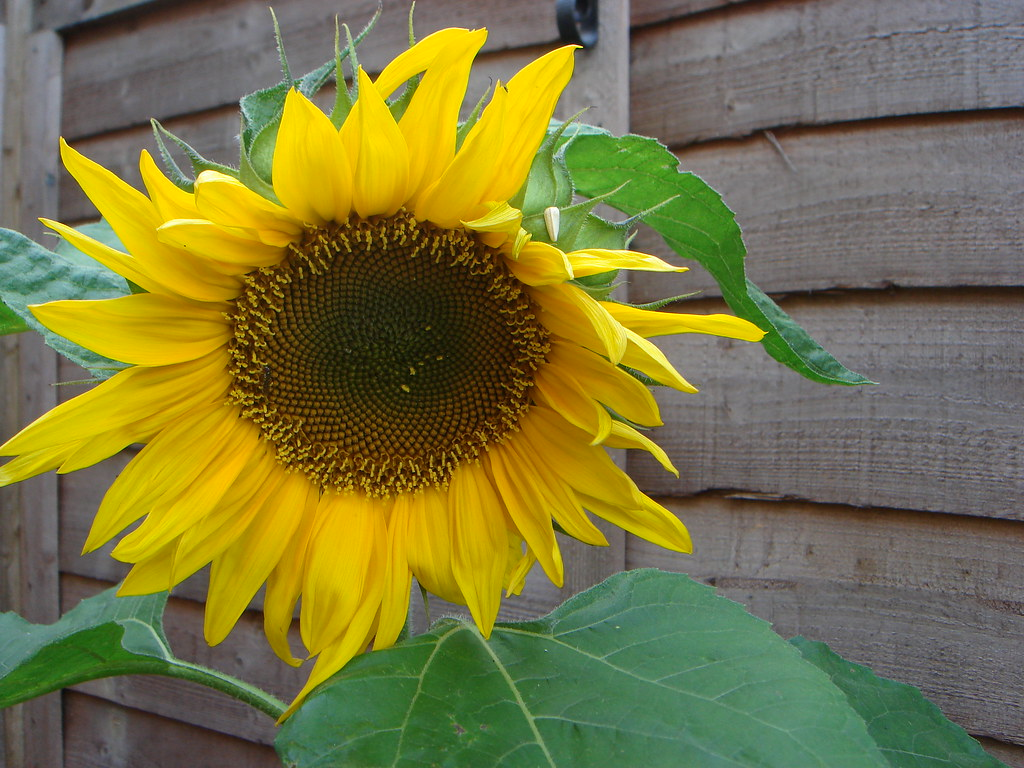
\includegraphics[width=7cm]{sunflower.jpg}
\caption{\label{sunflower}Distribution of the seeds of a sunflower (see \cite{simonbrassCCSearch2006} licenced under CC)}
\end{figure}

\subsection{Relating The Fibonacci Sequence to the Julia Set}
\label{sec:org4b34668}
See \href{https://youtu.be/ovJcsL7vyrk}{this link}.
\section{Julia Sets}
\label{sec:orgd203cf7}

The julia set is the outline \cite[Ch. 14]{peitgenChaosFractalsNew2004}.

The mandelbrot has to do with whether or not it's connected.
,** TODO The math behind it
,*** TODO Like Escaping after 2
I cannot figure this out, I need more time, look around Ch. 12 of falconer \cite{falconerFractalGeometryMathematical2003}
There is a relatioship between the fibonacicci sequence, modelling population growth and the mandelbrot curve, I would like to use that to tie some of the discussion together, see \href{https://youtu.be/ovJcsL7vyrk}{this video from Veritasium to get an idea of what i mean}.


\subsection{Introduction}
\label{sec:org8e05b05}
Julia sets are a very interesting fractal and we hope to investigate them further in this project.
\subsection{Motivation}
\label{sec:orgf9d4041}
Consider the iterative process \(x \rightarrow x^{2}, \enspace x \in \mathbb{R}\),
for values of \(x>1\) this process will diverge and for \(x<1\) it will converge.

Now Consider the iterative process \(z \rightarrow z^{2}, \enspace z \in \mathbb{C}\),
for values of \(\left\lvert z \right\rvert >1\) this process will diverge and for \(\left\lvert z \right\rvert <1\) it will converge.

Although this seems trivial this can be generalised.

Consider:

\begin{itemize}
\item The complex plane for \(\left\lvert z \right\rvert \leq 1\)
\item Some function \(f_{c}(z) = z^{2} + c, \quad c \leq 1 \in \mathbb{C}\) that can be used to iterate with
\end{itemize}

Every value on that plane will belong to one of the two following sets

\begin{itemize}
\item \(P_{c}\)
\begin{itemize}
\item The set of values on the plane that converge to zero (prisoners)
\item Define \(Q^{(k)}_{c}\) to be the the set of values confirmed as prisoners after \(k\) iterations of \(f_{c}\)
\begin{itemize}
\item this implies \(\lim_{k \rightarrow \infty} \left[ Q^{(k)}_{c}  \right] = P_{c}\)
\end{itemize}
\end{itemize}
\item \(E_{c}\)
\begin{itemize}
\item The set of values on the plane that tend to \(\infty\) (escapees)
\end{itemize}
\end{itemize}

In the case of \(f_{0}(z) = z^{2}\) all values \(\left\lvert z  \right \rvert \leq 1\) are bounded with \(\left\lvert z  \right \rvert = 1\) being an unstable stationary circle, but let's investigate what happens for different iterative functions like \(f_{1}(z) = z^{2} - 1\), despite how trivial this seems at first glance.

\subsection{Plotting the Sets}
\label{sec:org8b25ab6}
Although the convergence of values may appear simple at first, we'll implement a
strategy to plot the prisoner and escape sets on the complex plane.

Because this involves iteration and \emph{Python} is a little slow, We'll denote
complex values as a vector\footnote{See figure for the obligatory \emph{XKCD} Comic} and define the operations as described in
listing \ref{complex-vec}.\footnote{This technique was adapted from Chapter 7 of \emph{Math adventures with Python} \cite{farrellMathAdventuresPython2019}}

To implement this test we'll consider a function called \texttt{escape\_test} that applies an
iteration (in this case \(f_{0}: z \rightarrow z^{2}\)) until that value diverges or converges.

While iterating with \(f_{c}\) once \(\left\lvert z \right\rvert >
\mathrm{max}\left(\left\{c, 2\}\right)\), the value must diverge because
\(\left\lvert c \rvert\right \leq 1\), so rather than record whether or not the
value converges or diverges, the \texttt{escape\_test} can instead record the number of
iterations \((k)\) until the value has crossed that boundary and this will provide
a measurement of the rate of divergence.

Then the \texttt{escape\_test} function can be mapped over a matrix, where each element
of that matrix is in turn mapped to a point on the cartesian plane, the resulting matrix
can be visualised as an image \footnote{these cascading values are much like brightness in Astronomy}, this is implemented in listing
\ref{py-circle-code} and the corresponding output shown in \ref{py-circle-plot}.

with respect to listing \ref{py-circle-code}:

\begin{itemize}
\item Observe that the \texttt{magnitude} function wasn't used:
\begin{enumerate}
\item This is because a \texttt{sqrt} is a costly operation and comparing two squares saves an operation
\end{enumerate}
\end{itemize}



\begin{listing}[htbp]
\begin{minted}[]{python}
from math import sqrt
def magnitude(z):
    # return sqrt(z[0]**2 + z[1]**2)
    x = z[0]
    y = z[1]
    return sqrt(sum(map(lambda x: x**2, [x, y])))

def cAdd(a, b):
    x = a[0] + b[0]
    y = a[1] + b[1]
    return [x, y]


def cMult(u, v):
    x = u[0]*v[0]-u[1]*v[1]
    y = u[1]*v[0]+u[0]*v[1]
    return [x, y]
\end{minted}
\caption{\label{complex-vec}Defining Complex Operations with vectors}
\end{listing}

\begin{listing}[htbp]
\begin{minted}[]{python}
%matplotlib inline
%config InlineBackend.figure_format = 'svg'
import numpy as np
def escape_test(z, num):
    ''' runs the process num amount of times and returns the count of
    divergence'''
    c = [0, 0]
    count = 0
    z1 = z  #Remember the original value that we are working with
    # Iterate num times
    while count <= num:
        dist = sum([n**2 for n in z1])
        distc = sum([n**2 for n in c])
        # check for divergence
        if dist > max(2, distc):
            #return the step it diverged on
            return count
        #iterate z
        z1 = cAdd(cMult(z1, z1), c)
        count+=1
        #if z hasn't diverged by the end
    return num



p = 0.25 #horizontal, vertical, pinch (zoom)
res = 200
h = res/2
v = res/2

pic = np.zeros([res, res])
for i in range(pic.shape[0]):
    for j in range(pic.shape[1]):
        x = (j - h)/(p*res)
        y = (i-v)/(p*res)
        z = [x, y]
        col = escape_test(z, 100)
        pic[i, j] = col

import matplotlib.pyplot as plt

plt.axis('off')
plt.imshow(pic)
# plt.show()

\end{minted}
\caption{\label{py-circle-code}Circle of Convergence of \(z\) under recursion}
\end{listing}


\begin{figure}[htbp]
\centering
\includesvg[width=9cm]{circle-of-convergence}
\caption{\label{py-circle-plot}Circle of Convergence for \(f_{0}: z \rightarrow z^{2}\)}
\end{figure}

This is precisely what we expected, but this is where things get interesting,
consider now the result if we apply this same procedure to \(f_{1}: z \rightarrow
z^{2} - 1\) or something arbitrary like \(f_{\frac{1}{4} + \frac{i}{2}}: z
\rightarrow z^{2} + (\frac{1}{4} + \frac{i}{2})\), the result is something
remarkebly unexpected, as shown in figures \ref{py-jl-1-plot} and \ref{py-jl-rab-plot}.


\begin{figure}[htbp]
\centering
\includesvg[width=9cm]{./julia-1}
\caption{\label{py-jl-1-plot}Circle of Convergence for \(f_{0}: z \rightarrow z^{2} - 1\)}
\end{figure}


\begin{figure}[htbp]
\centering
\includesvg[width=9cm]{./julia-rab}
\caption{\label{py-jl-rab-plot}Circle of Convergence for \(f_{\frac{1}{4} + \frac{i}{2}}: z \rightarrow z^{2} + \frac{1}{4} + \frac{i}{2}\)}
\end{figure}

To investigate this further consider the
more general function \(f_{0.8 e^{\pi i \tau}}: z \rightarrow z^{2} + 0.8 e^{\pi
i \tau}, \enspace \tau \in \mathbb{R}\), many fractals can be generated using
this set by varying the value of \(\tau\)\footnote{This approach was inspired by an animation on the \emph{Julia Set} Wikipedia article \cite{JuliaSet2020}}.

\emph{Python} is too slow for this, but the \emph{Julia} programming language, as a
compiled language, is significantly faster and has the benefit of treating
complex numbers as first class citizens, these images can be generated in
\emph{Julia} in a similar fashion as before, with the specifics shown in listing
\ref{julia-gen-fracs}. The \texttt{GR} package appears to be the best plotting library
performance wise and so was used to save corresponding images to disc, this is
demonstrated in listing \ref{GR-save} where 1200 pictures at a 2.25 MP resolution were produced. \footnote{On my system this took about 30 minutes.}

A subset of these images can be combined using \emph{ImageMagick} and \texttt{bash} to
create a collage, \emph{ImageMagick} can also be used to produce an animation but it often
fails and a superior approach is to use \texttt{ffmpeg}, this is demonstrated in
listing \ref{bash-frac-join}, the collage is shown in figure \ref{montage-frac} and a corresponding
animation is \href{https://dl.dropboxusercontent.com/s/rbu25urfg8sbwfu/out.gif?dl=0}{available online}\footnote{\href{https://dl.dropboxusercontent.com/s/rbu25urfg8sbwfu/out.gif?dl=0}{https://dl.dropboxusercontent.com/s/rbu25urfg8sbwfu/out.gif?dl=0}}].

\begin{listing}[htbp]
\begin{minted}[]{julia}
# * Define the Julia Set
"""
Determine whether or not a value will converge under iteration
"""
function juliaSet(z, num, my_func)
    count = 1
    # Remember the value of z
    z1 = z
    # Iterate num times
    while count ≤ num
        # check for divergence
        if abs(z1)>2
            return Int(count)
        end
        #iterate z
        z1 = my_func(z1) # + z
        count=count+1
    end
        #if z hasn't diverged by the end
    return Int(num)
end

# * Make a Picture
"""
Loop over a matrix and apply apply the julia-set function to
the corresponding complex value
"""
function make_picture(width, height, my_func)
    pic_mat = zeros(width, height)
    zoom = 0.3
    for i in 1:size(pic_mat)[1]
        for j in 1:size(pic_mat)[2]
            x = (j-width/2)/(width*zoom)
            y = (i-height/2)/(height*zoom)
            pic_mat[i,j] = juliaSet(x+y*im, 256, my_func)
        end
    end
    return pic_mat
end

\end{minted}
\caption{\label{julia-gen-fracs}Produce a series of fractals using julia}
\end{listing}

\begin{listing}[htbp]
\begin{minted}[]{julia}
# * Use GR to Save a Bunch of Images
  ## GR is faster than PyPlot
using GR
function save_images(count, res)
    try
        mkdir("/tmp/gifs")
    catch
    end
    j = 1
    for i in (1:count)/(40*2*π)
        j = j + 1
        GR.imshow(make_picture(res, res, z -> z^2 + 0.8*exp(i*im*9/2))) # PyPlot uses interpolation = "None"
        name = string("/tmp/gifs/j", lpad(j, 5, "0"), ".png")
        GR.savefig(name)
    end
end

save_images(1200, 1500) # Number  and Res
\end{minted}
\caption{\label{GR-save}Generate and save the images with GR}
\end{listing}

\begin{listing}[htbp]
\begin{minted}[]{bash}
# Use montage multiple times to get recursion for fun
montage (ls *png | sed -n '1p;0~600p') 0a.png
montage (ls *png | sed -n '1p;0~100p') a.png
montage (ls *png | sed -n '1p;0~50p') -geometry 1000x1000  a.png

# Use ImageMagick to Produce a gif (unreliable)
convert -delay 10 *.png 0.gif

# Use FFMpeg to produce a Gif instead
ffmpeg                    \
    -framerate 60         \
    -pattern_type glob    \
    -i '*.png'            \
    -r 15                 \
    out.mov


\end{minted}
\caption{\label{bash-frac-join}Using \texttt{bash}, \texttt{ffmpeg} and \emph{ImageMagick} to combine the images and produce an animation.}
\end{listing}

\url{\_20200826\_005334a.png}

\section{MandelBrot Set}
\label{sec:org4275c56}
Investigating these fractals, a natural question might be whether or not any
given \(c\) value will produce a fractal that is an open disc or a closed disc.

So pick a value \(\left\lvert \gamma \right \rvert < 1\) in the complex plane and
use it to produce the julia set \(f_{\gamma}\), if the corresponding prisoner set
\(P\) is closed we this value is defined as belonging to the \emph{Mandelbrot} set.

It can be shown (and I intend to show it generally), that this set is equivalent to re-implementing the previous strategy such that \(z \rightarrow z^{2} + z_{0}\) where \(z_{0}\) is unchanging or more clearly as a seqeuence:

\begin{align}
z_{n+1} &= z^{2}_n + c \label{eq:mb-sequence} \\
z_{0}   &= c
\end{align}

This strategy is implemented in listing and produces the output shown in figure \ref{mandelbrot-py-pic}.

\begin{listing}[htbp]
\begin{minted}[]{python}
%matplotlib inline
%config InlineBackend.figure_format = 'svg'
def mandelbrot(z, num):
    ''' runs the process num amount of times and returns the count of
    divergence'''
    count = 0
    # Define z1 as z
    z1 = z
    # Iterate num times
    while count <= num:
        # check for divergence
        if magnitude(z1) > 2.0:
            #return the step it diverged on
            return count
        #iterate z
        z1 = cAdd(cMult(z1, z1),z)
        count+=1
        #if z hasn't diverged by the end
    return num

import numpy as np


p = 0.25 # horizontal, vertical, pinch (zoom)
res = 200
h = res/2
v = res/2

pic = np.zeros([res, res])
for i in range(pic.shape[0]):
    for j in range(pic.shape[1]):
        x = (j - h)/(p*res)
        y = (i-v)/(p*res)
        z = [x, y]
        col = mandelbrot(z, 100)
        pic[i, j] = col

import matplotlib.pyplot as plt
plt.imshow(pic)
# plt.show()
\end{minted}
\caption{\label{py-mandelbrot-code}All values of \(c\) that lead to a closed \emph{Julia-set}}
\end{listing}

\begin{figure}[htbp]
\centering
\includesvg[width=8cm]{./mandelbrot-py}
\caption{\label{mandelbrot-py-pic}Mandelbrot Set produced in \emph{Python} as shown in listing \ref{py-mandelbrot-code}}
\end{figure}

This output although remarkable is however fairly undetailed, by using \emph{Julia} a much
larger image can be produced, in \emph{Julia} producing a 4 GB, 400 MP image can be done in little time
(about 10 minutes on my system), this is demonstrated in listing 
and the corresponding FITS image is \href{https://www.dropbox.com/s/jd5qf1pi2h68f2c/mandelbrot-400mpx.fits?dl=0}{available-online.}\footnote{\href{https://www.dropbox.com/s/jd5qf1pi2h68f2c/mandelbrot-400mpx.fits?dl=0}{https://www.dropbox.com/s/jd5qf1pi2h68f2c/mandelbrot-400mpx.fits?dl=0}}

\begin{minted}[]{julia}
function mandelbrot(z, num, my_func)
    count = 1
    # Define z1 as z
    z1 = z
    # Iterate num times
    while count ≤ num
        # check for divergence
        if abs(z1)>2
            return Int(count)
        end
        #iterate z
        z1 = my_func(z1) + z
        count=count+1
    end
        #if z hasn't diverged by the end
    return Int(num)
end

function make_picture(width, height, my_func)
    pic_mat = zeros(width, height)
    for i in 1:size(pic_mat)[1]
        for j in 1:size(pic_mat)[2]
            x = j/width
            y = i/height
            pic_mat[i,j] = mandelbrot(x+y*im, 99, my_func)
        end
    end
    return pic_mat
end


using FITSIO
function save_picture(filename, matrix)
    f = FITS(filename, "w");
    # data = reshape(1:100, 5, 20)
    # data = pic_mat
    write(f, matrix)  # Write a new image extension with the data

    data = Dict("col1"=>[1., 2., 3.], "col2"=>[1, 2, 3]);
    write(f, data)  # write a new binary table to a new extension

    close(f)
end

# * Save Picture
#------------------------------------------------------------
my_pic = make_picture(20000, 20000, z -> z^2) 2000^2 is 4 GB
save_picture("/tmp/a.fits", my_pic)

\end{minted}

\begin{figure}[htbp]
\centering
\includegraphics[width=10cm]{_20200828_233844screenshot.png}
\caption{\label{mandelbrot-screen}Screenshot of Mandelbrot FITS image produced by listing }
\end{figure}
\section{Appendix}
\label{appendix}
So unless code contributes directly to the discussion we'll put it in the appendix.
\subsection{Finding Material}
\label{sec:orgf40070f}
\begin{minted}[]{bash}
recoll -c /home/ryan/Dropbox/Books/Textbooks/Mathematics/Chaos_Theory/chaos_books_recoll & disown
\end{minted}
\subsection{Font Lock}
\label{sec:org4d0319e}
\begin{minted}[]{elisp}
;; match:
;;; \scite:key\s
(add-to-list 'font-lock-extra-managed-props 'display)
(font-lock-add-keywords nil
 '((" \\(cite:[a-z0-9A-Z]\+\\)" 1 '(face nil display "🤔"))))


;; match
;;; [[cite:key][p. num]]
(add-to-list 'font-lock-extra-managed-props 'display)
(font-lock-add-keywords nil
 '((" \\(\\[\\[cite:[a-z0-9A-Z]\+\\]\\[\.\*\\]\\]\\)" 1 '(face nil display "🤔"))))
\end{minted}
\subsection{Resources Used for the Hausdorff Dimension}
\label{haus-resource}
Research for \S \ref{Hausdorff-dimension} on the Hausdorff Dimension proved actually to be quite difficult, while much information is available online, precice and clear explanations of the Hausdorff dimension are difficult to find without scouring texts, the following proved very helpful generally in preparing for this topic and I would strongly recommend these chapters as a starting point for further reading on this topic:

\begin{itemize}
\item Edgar, G. A., \emph{Measure, topology, and fractal geometry} \cite[Ch. 6]{edgarMeasureTopologyFractal2008a}
\item Falconer, K. J., \emph{Fractal geometry: mathematical foundations and applications}  \cite[Ch. 2]{falconerFractalGeometryMathematical2003b}
\item Gouyet, J., \emph{Physics and fractal structures} \cite[\S1.3]{gouyetPhysicsFractalStructures1996}
\item Vicsek, T., \emph{Fractal Growth Phenomena} \cite[Ch. 4]{vicsekFractalGrowthPhenomena1992}
\begin{itemize}
\item See also p 14 specifically
\end{itemize}
\item Tél, T., Gruiz, M., \& Kulacsy, K., \emph{Chaotic dynamics: an introduction based on classical mechanics}  \cite[\S2.1.2]{telChaoticDynamicsIntroduction2006}
\item Peitgen, H., Jürgens, H., \& Saupe, D., \emph{Chaos and fractals: new frontiers of science}  \cite[\S 4.3]{peitgenChaosFractalsNew2004}
\end{itemize}
\end{document}
